\documentclass[11pt,center]{beamer}

\usepackage{fancybox}
\usepackage{graphicx}
\usepackage{spot}
\usepackage{minibox}
\usepackage[absolute,overlay]{textpos}
\usepackage[backend=biber, style=numeric, %citestyle=authoryear, maxcitenames=1,
			isbn=false,doi=false]{biblatex}
\usetheme{metropolis}

\usepackage[export]{adjustbox}

\newcommand{\mli}[1]{\mathit{#1}}

%---		BIBLIOGRAPHY		---%
\bibliography{../../bib/primary.bib}
\DefineBibliographyStrings{english}{
  references = {Αναφορές},
}
\setbeamertemplate{bibliography item}[text]
\renewcommand*{\bibfont}{\scriptsize}
\setbeamerfont{footnote}{size=\tiny}

\definecolor{light-gray}{gray}{0.86}
\title{\huge{Adaptive Machine Learning} \newline \large{Observing the regularities in the world}}
\author{Βασίλειος Αταλόγλου \newline Κωνσταντίνος Σαμαράς-Τσακίρης}
\date{\today}

\begin{document}

\begin{frame}%{\maketitle}
  \titlepage
\end{frame}

% Intro
\begin{frame}
  %Ο κόσμος παράγει δεδομένα. Τα αισθανόμαστε: ροές δεδομένων.
  %Τα δεδομένα αλλάζουν. Παράδειγμα ρομπότ;
  \centering
  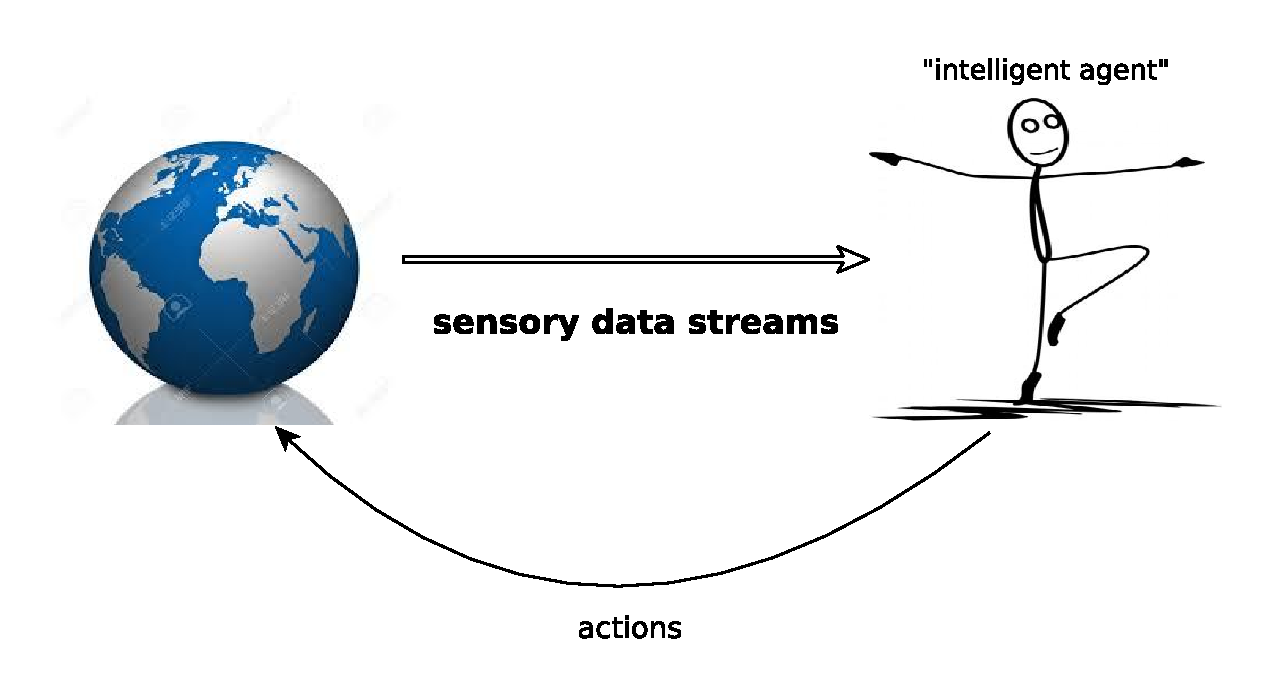
\includegraphics[width=0.8\textwidth]{../pics/world-man-interaction}
  \only<1-6>{\visible<2-6>{
    \begin{itemize}[<+(1)->]
      \item Βλέπει κι ακούει τον κόσμο και δρα πάνω του
      \item Δέχεται \alert{αλληλουχίες} ερεθισμάτων και ανιχνεύει \alert{συνεπακόλουθα}
      \item Μαθαίνει τη δομή και τις βασικές αρχές του
      \item ``Κοινή λογική''
      \item[] Και αυτά με τρόπο \emph{unsupervised}, πραγματοποιώντας διαρκώς \emph{προβλέψεις}.
    \end{itemize}
  }}
  \only<7->{ 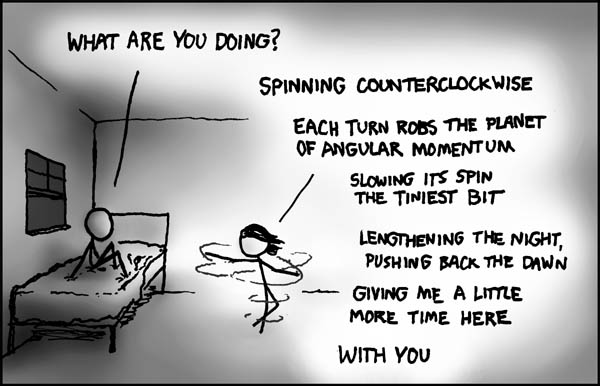
\includegraphics[width=0.65\textwidth]{../pics/angular_momentum} }
\end{frame}

\begin{frame}{Beyond the static \& supervised \tiny{\cite{lecun,staticbottleneck}}}
  %Στατική και supervised μάθηση δεν αρκεί. Πρόβλημα: αναγνώριση προτύπων σε ροές δεδομένων, sequence learning
  \begin{block}{Μοντελοποιώντας έναν κόσμο που αλλάζει}
    \pause
    \vspace{-0.5em}
    \begin{itemize}
      \item Το μοντέλο πρέπει ή να είναι γενικό ή να προσαρμόζεται
      \item Δεν είναι δυνατό να δημιουργηθούν labeled datasets -- υπερβολικός κόπος ή άγνοια
        \pause
      \item Τα δεδομένα έρχονται σε χρονική αλληλουχία \\ $\rightarrow$ Αιτιώδεις σχέσεις
    \end{itemize}
  \end{block}

  \pause
  \vspace{-0.5em}
  \begin{block}{Πρόβλημα: Sequence learning}
    Ο πράκτορας παρακολουθεί μια ακολουθία δεδομένων και καλείται να προβλέψει τη συνέχεια και να δράσει έτσι, ώστε να ανταμειφθεί. \\
    Κατ'επέκταση:
    \vspace{-0.3em}
    \begin{itemize}
      \item Αναγνώριση ανωμαλίας
      \item Λήψη αποφάσεων (κίνητρο παρέχεται από το περιβάλλον)
    \end{itemize}
  \end{block}
\end{frame}

\begin{frame}{How to do sequence learning}
  \begin{columns}
    \column{0.5\textwidth}
    \begin{itemize}
      \item<2-> Hidden markov model
      \item<3-> Time-delay neural network
      \item<4-> Recurrent neural network
        \begin{itemize}
          \item[--] LSTM
        \end{itemize}
    \end{itemize}
    \visible<5->{
      \centering
    \vspace{25pt}
    \em\Large{Γενικότερο μοντέλο;}
    }
    \column{0.5\textwidth}
    \begin{itemize}
      \item[]<2-> 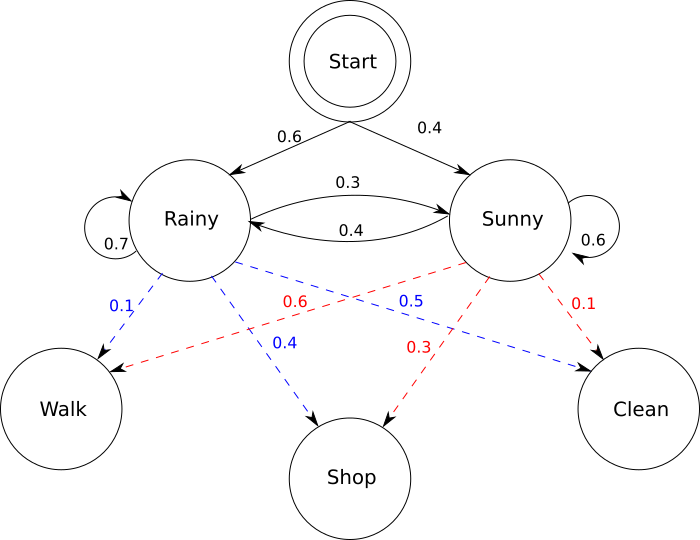
\includegraphics[width=0.8\textwidth]{../pics/hmm2}
      \item[]<4-> 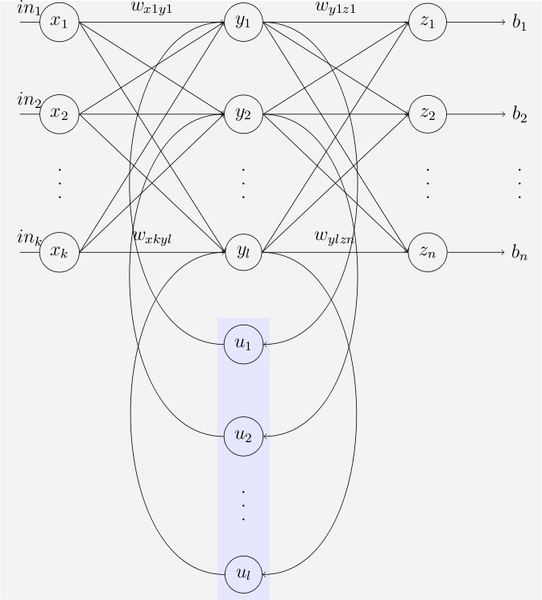
\includegraphics[width=0.74\textwidth]{../pics/rnn}
    \end{itemize}
  \end{columns}
\end{frame}

\begin{frame}{Ανθρώπινος εγκέφαλος}
  O άνθρωπος έχει \alert{μνήμη} και μαθαίνει \alert{συνεχώς}, χωρίς επίβλεψη από το περιβάλλον.

  \pause
  \begin{columns}
    \column{0.7\textwidth}
    \\ Οι διαστάσεις του ανθρώπινου εγκεφάλου:
    \small{
      \begin{itemize}
        \item[--] $10^{11}$ νευρώνες
        \item[--] $10^4$ συνάψεις/νευρώνα
        \item[--] $10$ σήματα/$sec$/σύναψη
          \vspace{+0.5em}
        \item Σύνολο: $10^{15}$ σήματα/$sec$
        \item Ισχύς: $25$ Watt
      \end{itemize}
    }
    \column{0.3\textwidth}
    \\
    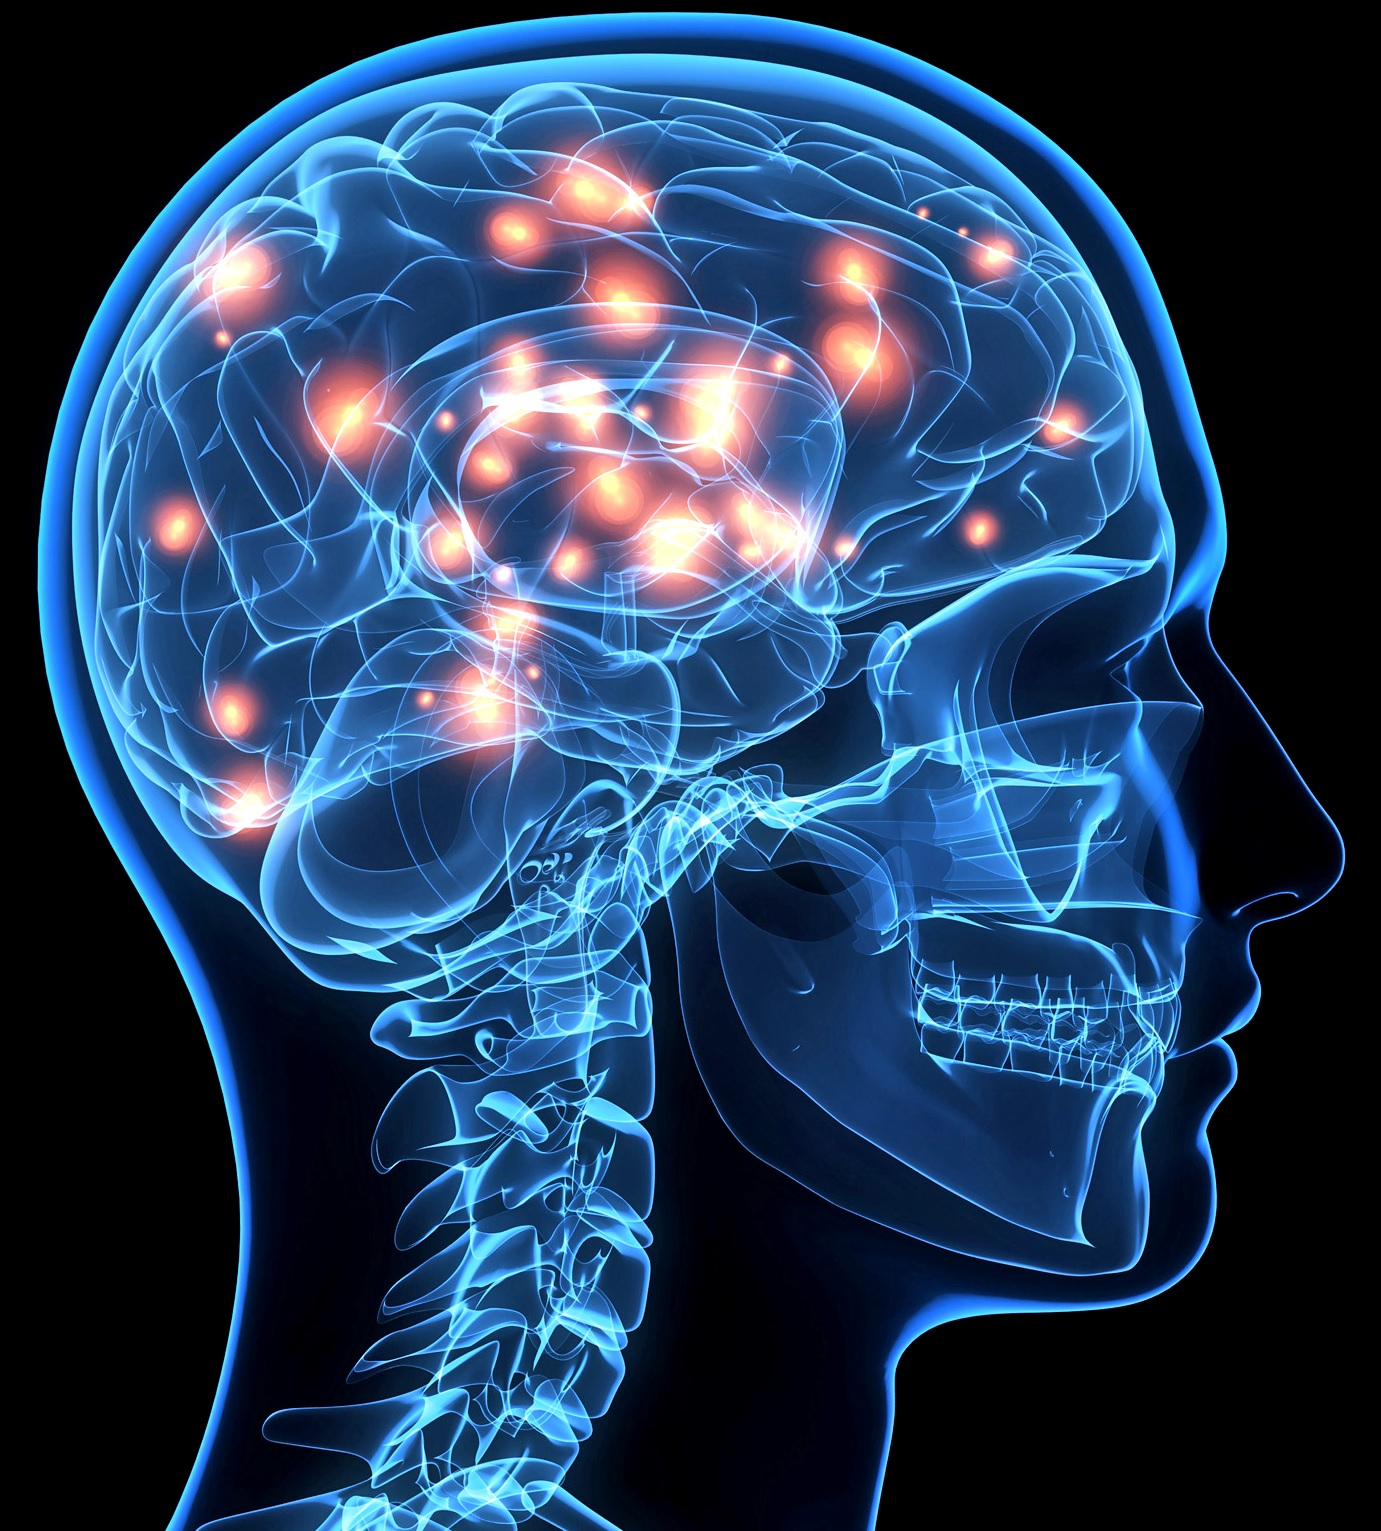
\includegraphics[width=1\textwidth]{../pics/brain.jpeg}
  \end{columns}

  \pause
  \begin{block}{}
    Οι δραστηριότητες που χαρακτηρίζουν τον άνθρωπο εντοπίζονται κυρίως στο \alert{neocortex}
  \end{block}
\end{frame}

\begin{frame}{Μοντελοποίηση λειτουργίας neocortex}
  Ανάγκη \alert{κατανόησης}
  \begin{itemize}
	\item Ο εγκέφαλος διαμορφώθηκε μέσω βιολογικής εξέλιξης και υπάγεται σε βιολογικούς περιορισμούς
	\item Ποιες είναι οι βασικές αρχές;
  \end{itemize}
  \visible<2->{
	Κάποιες παρατηρήσεις νευρολογίας neocortex:
	\begin{itemize}[]
	  \item<2-> Διδιάστατη μορφή χωρισμένη σε \alert{επίπεδα}
	  \item<3-> Δομή \alert{ομοιόμορφη} σε όλη του την έκταση
	  \begin{itemize} \item[--] Κάθε περιοχή λύνει το ίδιο πρόβλημα με τον ίδιο τρόπο \end{itemize}
		  \item<4-> Οι περιοχές ενώνονται \alert{ιεραρχικά}
		  \begin{itemize} \item[--] Ψηλότερα επίπεδα => πιο αφηρημένες έννοιες \end{itemize}
			  \item<5-> Οι νευρώνες ενεργοποιούνται σποραδικά και πολύ σπάνια
			  \begin{itemize} \item[--] Διάνυσμα κατάστασης: \spot<7>{\alert<5-6>{αραιό}} \end{itemize}
				  \item<6-> Συνεχής \alert{πρόβλεψη} του μέλλοντος
	\end{itemize}
  }
\end {frame}

\begin{frame}{Sparse Distributed Representation}
  \begin{block}{``Δομή δεδομένων του εγκεφάλου'' \tiny{\cite{neuronssynapses,sdrkanerva}}}
	\begin{itemize}
	  \item Μεγάλο, αραιό, δυαδικό διάνυσμα
	  \item Κάθε bit έχει σημασιολογικό \alert{νόημα}
	\end{itemize}
  \end{block}
\end{frame}

\begin{frame}{Ιδιότητες SDR}
  %\item Compressed storage
  %\item Similarity = intersection
  %\item Subsampling: 10 / 200
  %  \item Random match unlikely
  %  \item Partial match: generalization
  %\item Compare with union: set membership
  \begin{block}{Χωρητικότητα}
	Έστω το μέγεθος: $n$ και ο πληθυσμός των 1: $w$. Τα διαφορετικά SDRs με αυτή τη μορφή είναι $$ \binom nw= \frac{n!}{w!(n-w)!} $$
  \end{block}
  \pause
  \centering
  \vspace{1em}
  \large{Πώς μπορούμε να συνδυάσουμε/συγκρίνουμε δυο SDR?}
\end{frame}

\begin{frame}{Ταιριάζοντας SDRs}
  \only<1>{
	Έστω 2 SDR, το Α και το Β, ως δυαδικά διανύσματα:
	\begin{description}[Overlap set($b$)]
	  \item[Union] $A | B$
	  \item[Overlap] $A \& B$
	  \item[Overlap score] Το μέτρο του overlap
	  \item[Overlap set($b$)] Το σύνολο των SDR που έχουν overlap score $>b$ σε σχέση με το Α.
		\vspace{1em}
	  \item[Matching($\theta$)] Το Α και το Β ταιριάζουν, αν το overlap score τους είναι μεγαλύτερο από $\theta$
	\end{description}
  }
  \only<2->{
	\begin{itemize}
	  \item Έστω ότι Β = Α + 30\% θόρυβο. Τότε το εκτιμώμενο overlap score είναι $30\% \cdot w$. Αν $\theta = 30\% \cdot w$, τα Α και Β ταιριάζουν.
	  \item \alert{Ευρωστία} στο θόρυβο!
	  \item Πιθανότητα false positive: $8\times10^{-51}$ για $n=2048,\space w=41$
	\end{itemize}
	\pause
	$$p\{\mli{false\_positive}\}= \frac{|\mli{overlap\_set}|}{\mli{SDR\_capacity}}$$
  }
\end{frame}

\iffalse
\begin{frame} {Υποδειγματοληψία SDR}
  Συμπίεση: αποθηκεύονται μόνο θέσεις των 1

  \begin{block}{Υποδειγματοληψία}
    Έστω ότι αποθηκεύεται μόνο το 50\%.
    Αν συγκριθεί με τυχαίο SDR, η πιθανότητα false positive είναι πάρα πολύ μικρή.
  \end{block}
\end{frame}
\fi
\begin{frame} {Σύνολα από SDR}
  \begin{block}{Ερώτηση}
    Παρατηρούμε μια αλληλουχία από SDR. Πώς θα μάθουμε αν το ξεχωριστό SDR Β το έχουμε ξαναδεί; Και... γρήγορα;
  \end{block}

  \pause
  \vspace{1em}
  \begin{block}{Εύκολο!}
    Θα συγκρίνουμε το Β με την \alert{ένωση} όλων των SDR
  \end{block}

  \pause
  \vspace{0.5em}
  \centering
  
\includegraphics[width=.5\textwidth]{../pics/balance}
\end{frame}


\section{Hierarchical Temporal Memory}

\begin{frame}{Μοντέλο νευρώνα \tiny{\cite{neuronssynapses}}}
  %Neuron with context
  %Minicolumn, layer: predictions, inhibitions
  \centering
  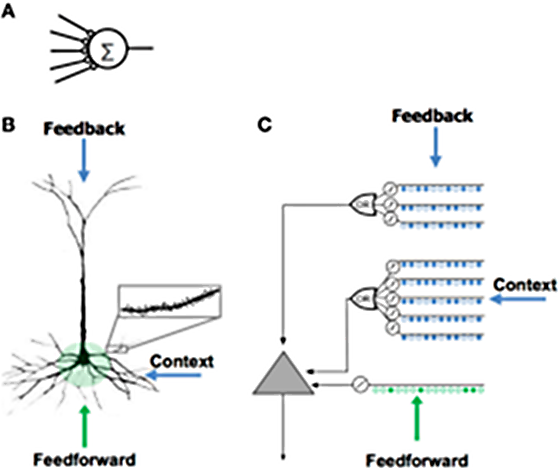
\includegraphics[width=.75\textwidth]{../pics/neuron-model}

  feedforward = receptive field
\end{frame}

\begin{frame}{Μοντέλο δικτύου}
  \centering
  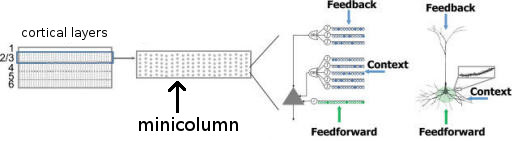
\includegraphics[width=.8\textwidth]{../pics/minicolumn}

  \vspace{-0.5em}
  \small{
    \begin{columns}
      \column{0.55\textwidth}
      \begin{block}{Συνάψεις}
        Νευρώνες στο ίδιο minicolumn
        \vspace{-0.5em}
        \begin{itemize}
          \item Tο ίδιο receptive field
          \item Μεταξύ τους inhibition
          \item[] $\rightarrow$ Winner-takes-all!
        \end{itemize}

        \vspace{-0.5em}
        Μεταξύ διαφορετικών minicolumns
        \vspace{-0.5em}
        \begin{itemize}
          \item Context
          \item Ολικό (ή τοπικό...) inhibition
        \end{itemize}
      \end{block}

      \column{0.45\textwidth}
      \begin{block}{Χαρακτηριστικά συνάψεων}
        \vspace{-0.5em}
        \begin{itemize}
          \item \alert{Υπάρχουν ή όχι}. Δε χρησιμοποιούνται βάρη.
          \item \emph{Μονιμότητα}: μια σύναψη με μικρή μονιμότητα μπορεί να απενεργοποιηθεί εύκολα
          \item Αλγόριθμοι μάθησης τύπου STDP
        \end{itemize}
      \end{block}
    \end{columns}
  }
\end{frame}

\begin{frame}{Scalar Encoder \tiny{\cite{htmschool}}}
  \only<1>{ 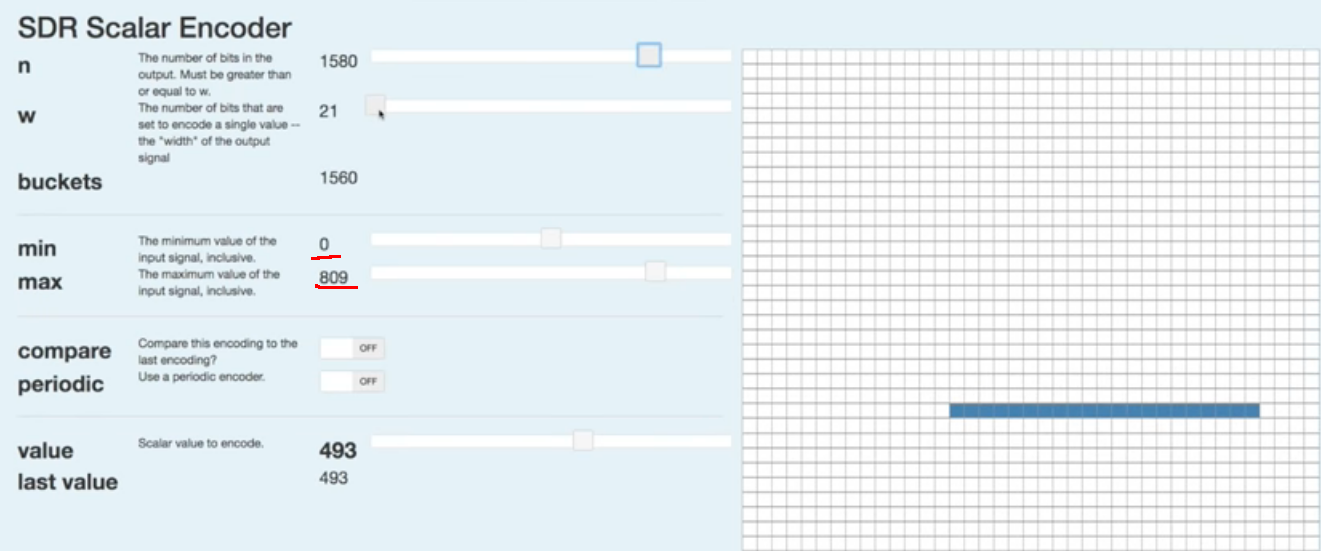
\includegraphics[width=1.05\textwidth]{../pics/enc1} }
  \only<2>{ 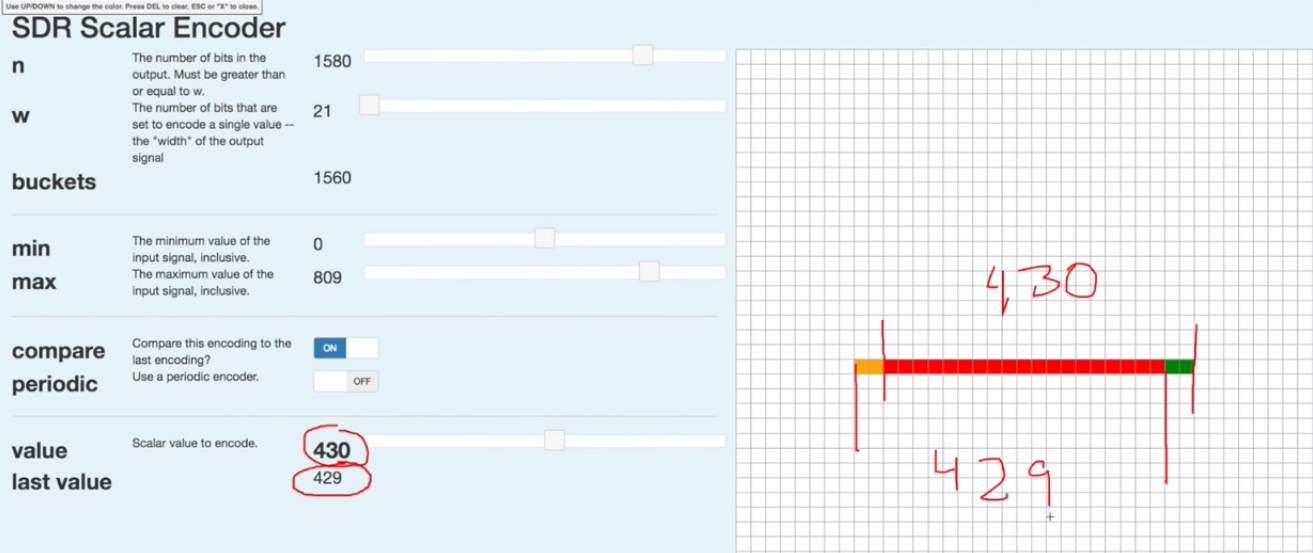
\includegraphics[width=1.05\textwidth]{../pics/enc2} }
  \only<3>{ 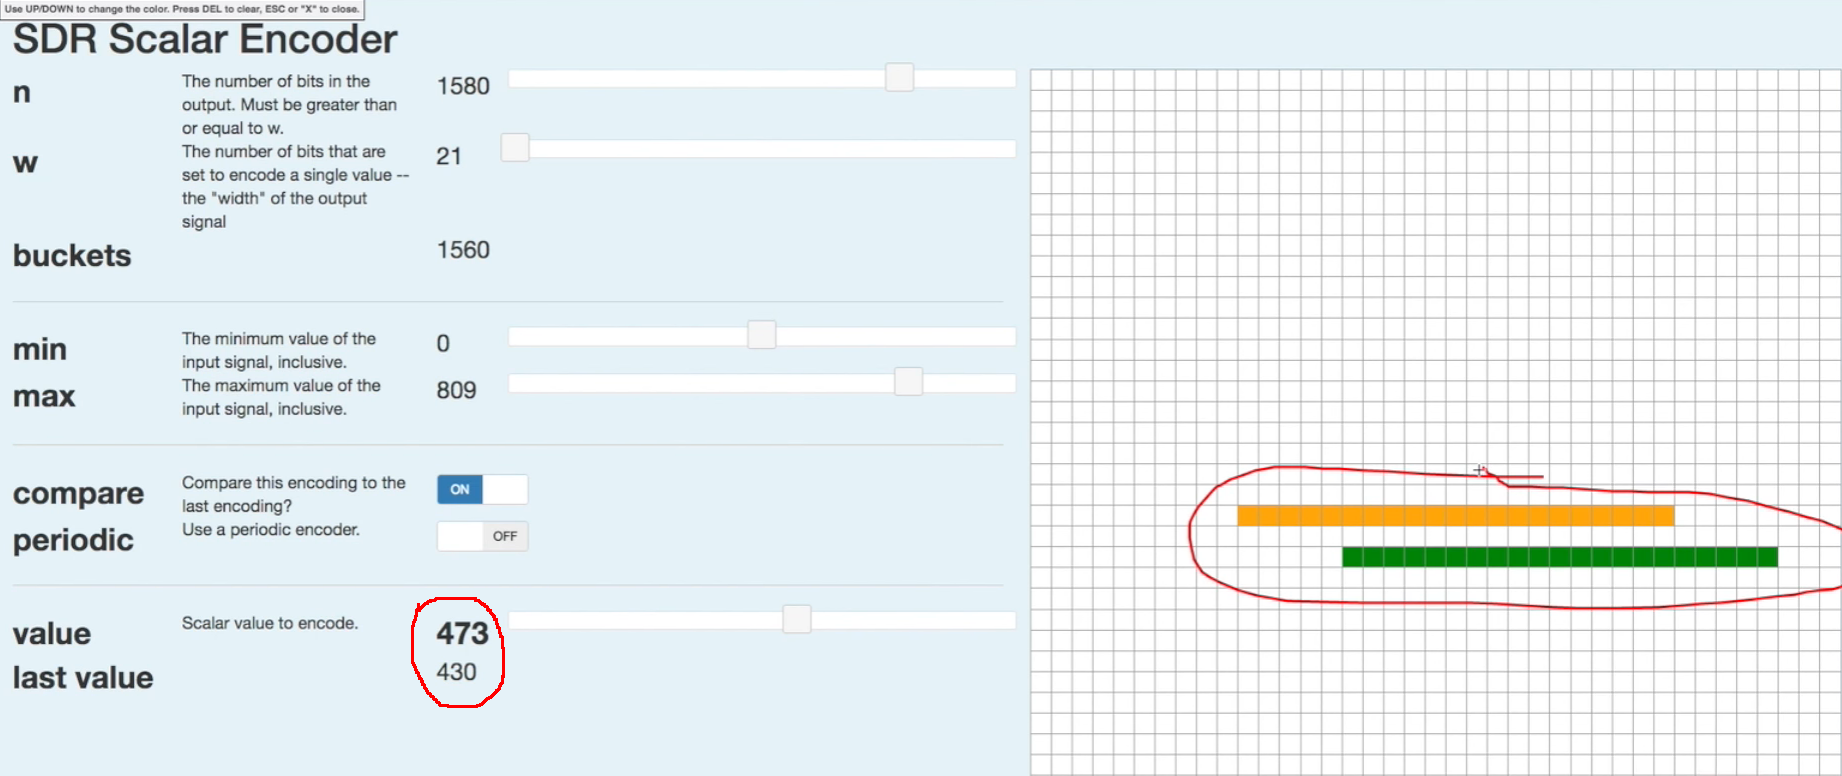
\includegraphics[width=1.05\textwidth]{../pics/enc3} }

  \only<1>{
    \begin{block}{Encoder}
      Οι ``αισθητήρες'' ενός συστήματος HTM. Εισάγουν τα ερεθίσματα του κόσμου.
    \end{block}}
\end{frame}

\begin{frame}{Text Encoder -- cortical.io}
  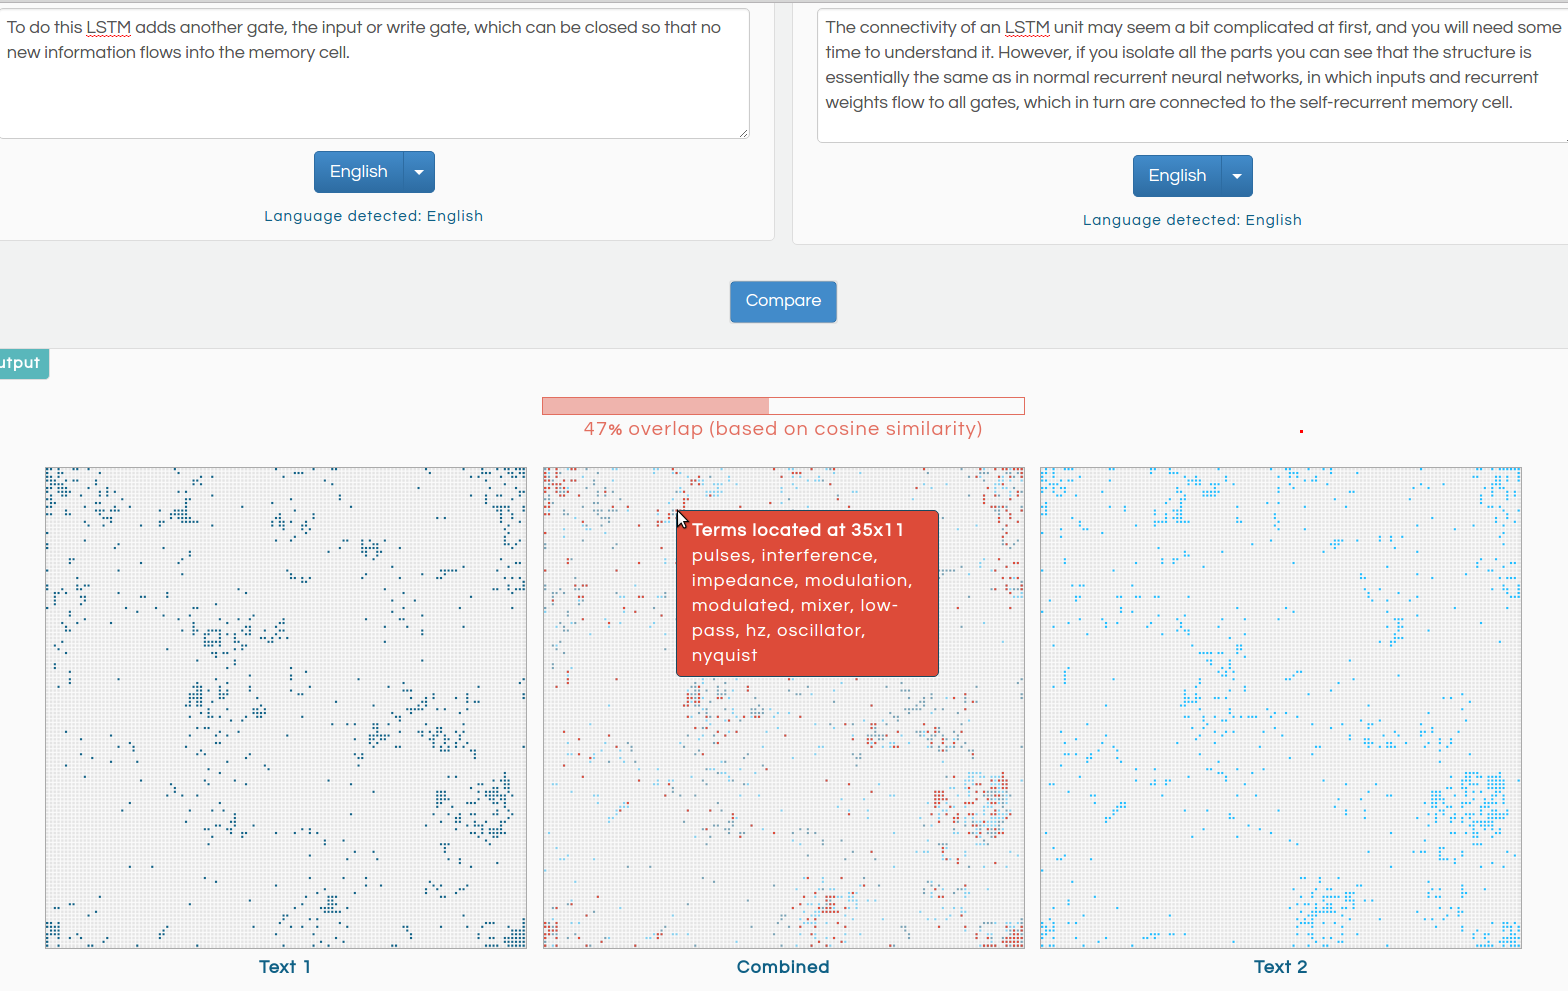
\includegraphics[width=1.05\textwidth]{../pics/enc-cortical}
\end{frame}


\section{Βασικές λειτουργίες HTM}

\begin{frame}{Spatial Pooler}
  \begin{block}{Spatial pooler}
    Επίπεδο HTM που κανονικοποιεί τα εισερχόμενα SDR, ρυθμίζοντας το μέγεθος, το sparsity ή την τοπολογία.
    Οφείλει να διατηρήσει τις \emph{ομοιότητες}.
    \begin{itemize}
      \item Δεν ενδιαφέρουν τα minicolumns εδώ
        %\item Κάθε νευρώνας συνδέεται τυχαία με μέρος της εισόδου
        %\item Οι νευρώνες που ενεργοποιούνται περισσότερο από την είσοδο νικούν
    \end{itemize}
  \end{block}

\end{frame}

\begin{frame}{Spatial Pooler \tiny{\cite{htmschool}}}
  \only<1>{ 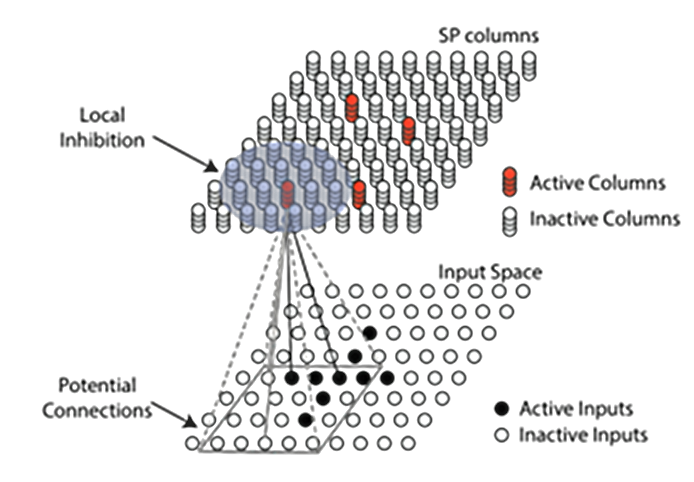
\includegraphics[width=1\textwidth]{../pics/spatpool} }
  \only<2>{ 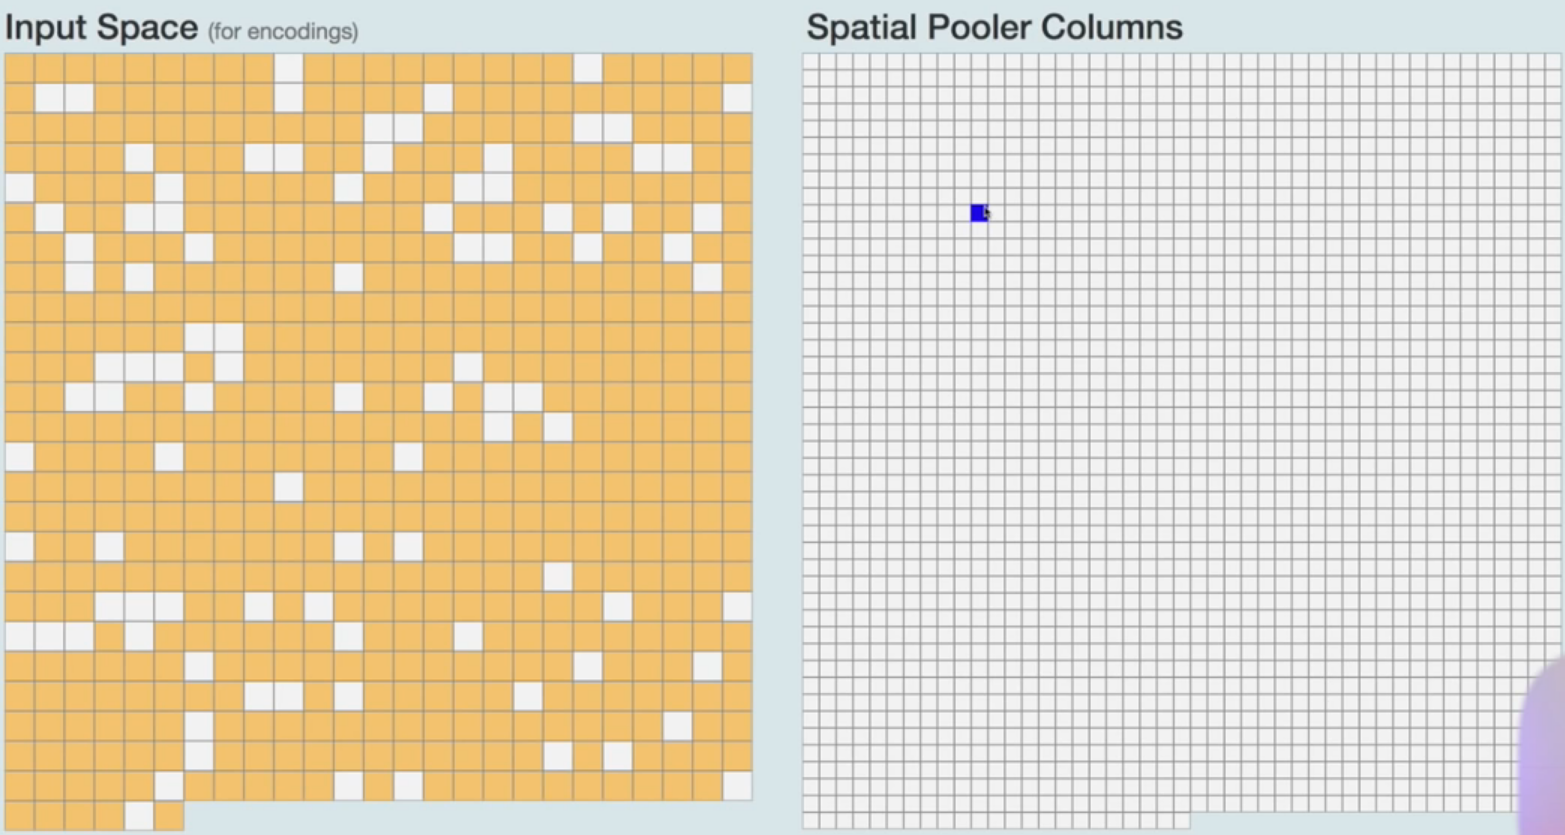
\includegraphics[width=1.07\textwidth]{../pics/sp1} }
  \only<3>{ 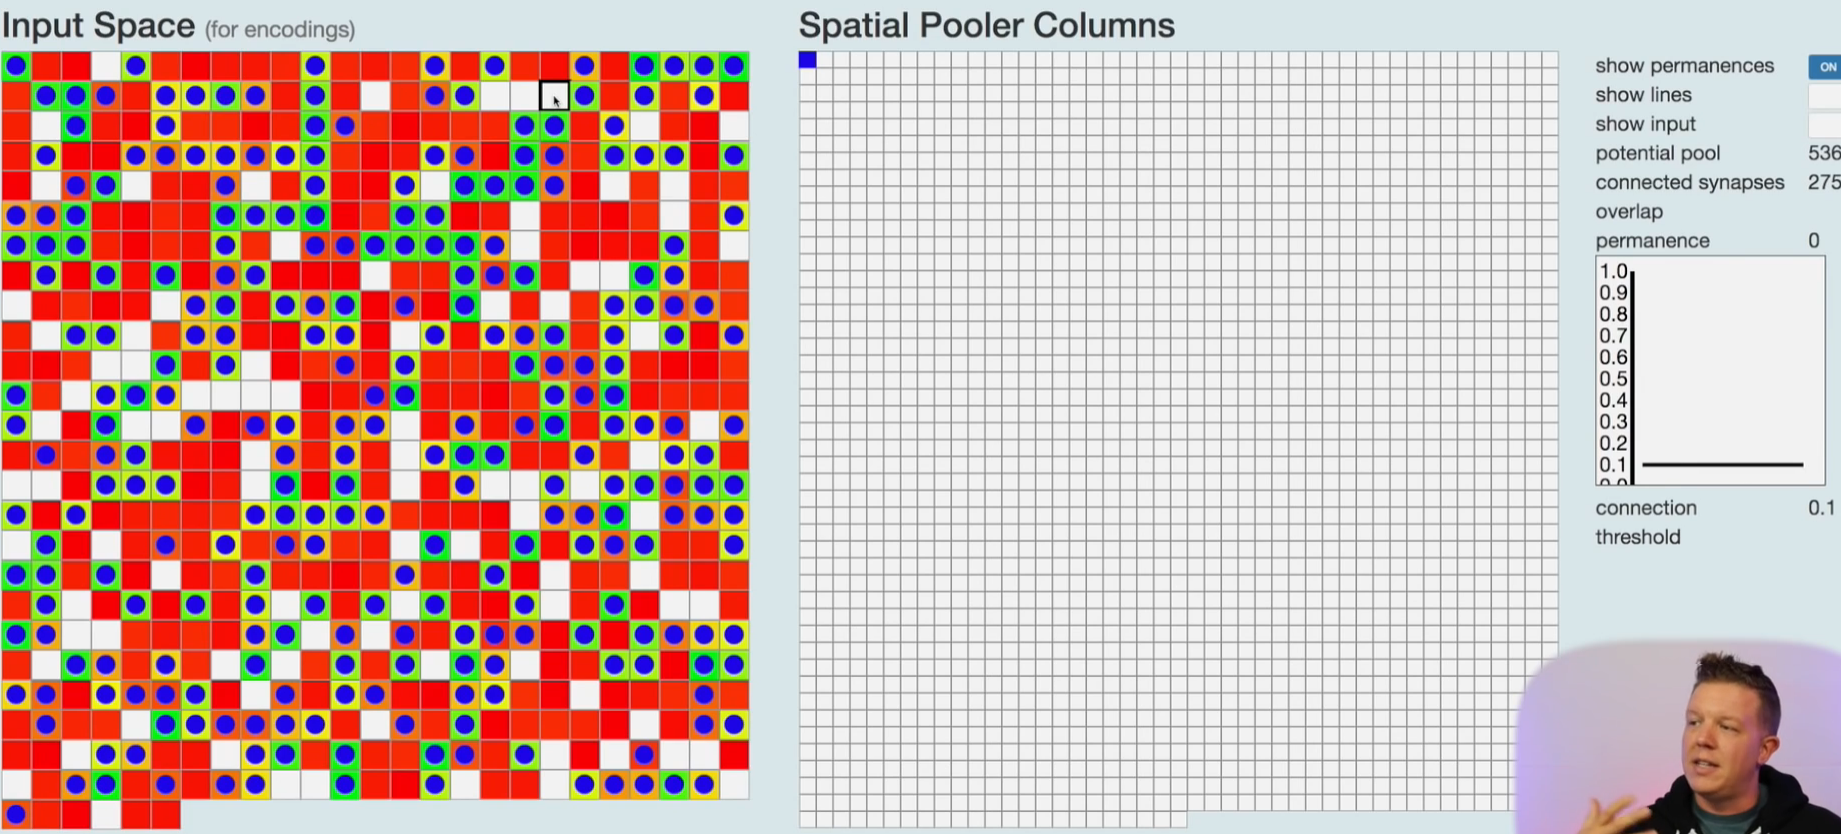
\includegraphics[width=1.07\textwidth]{../pics/sp2} }
\end{frame}

\begin{frame}{Sequence memory \tiny{\cite{neuronssynapses}}}
  \only<1>{ 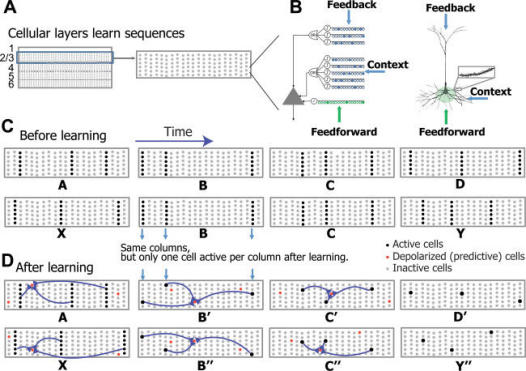
\includegraphics[width=0.95\textwidth]{../pics/sequence-learning-big} }
  \only<2>{ 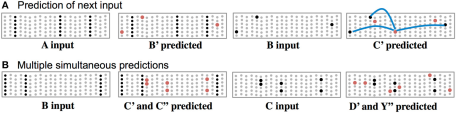
\includegraphics[width=1.05\textwidth]{../pics/sequence2} }
\end{frame}


\section{Προσομοιώσεις - Αποτελέσματα}

\begin{frame}{Τεχνητά δεδομένα}
  Δημιουργία set ακολουθιών \tiny{\cite{continuous,nab}}:
  \begin{itemize}
	\item[--]Απλή πρόβλεψη (A)
	\item[--]Πολλαπλή πρόβλεψη (B)
  \end{itemize}
  \vfill
  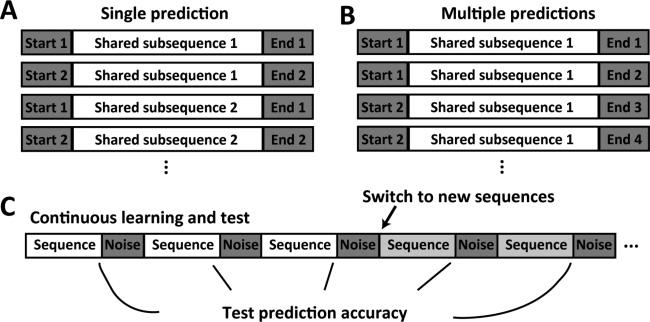
\includegraphics[width=0.6 \textwidth,center]{../pics/sequences.jpg}
  \vfill
  \pause
  Προσθήκη θορύβου ανάμεσα στις ακολουθίες
\end{frame}

\begin{frame}{Τεχνητά δεδομένα}
  Σύγκριση διαφορετικών υλοποιήσεων για μονή πρόβλεψη \tiny{\cite{continuous}}:\\
  \vspace{1em}
  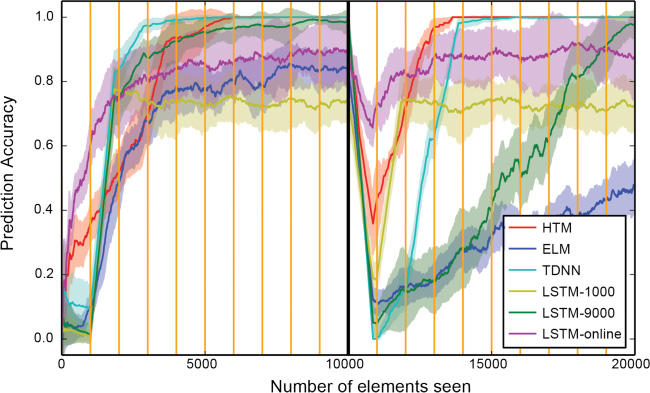
\includegraphics[width=0.7 \textwidth,center]{../pics/single_prediction.jpg}
  \pause
  \begin{tabbing}
	Το HTM:  \=α) πετυχαίνει perfect accuracy\\
	  \>β) προσαρμόζεται στις αλλαγές του περιβάλλοντος\\
  \end{tabbing}
\end{frame}

\begin{frame}{Τεχνητά δεδομένα}
  Πολλαπλές προβλέψεις:
  \vfill
  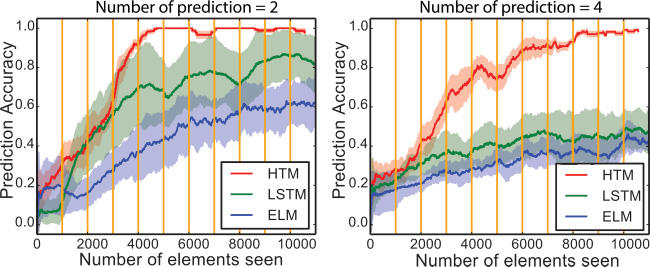
\includegraphics[width=0.7 \textwidth,center]{../pics/multiple_predictions.jpg}
  \pause
  \vfill
  To HTM είναι το \alert{μόνο} που πετυχαίνει perfect accuracy.\\
  \pause
  Αιτία: Αναπαράσταση με \textbf{SDR} !!
\end{frame}

\begin{frame}{Τεχνητά δεδομένα}
  \begin{columns}
	\column {0.4 \textwidth}
	\\
	\visible<1->{
	  Πρόβλεψη high-order ακολουθιών} \\
	\vspace{5em}
	\visible<2->{
	  Ανθεκτικότητα σε κατεστραμμένο δίκτυο}
	\column {0.6 \textwidth}
	\vspace{1em}
	\visible<1->{
	  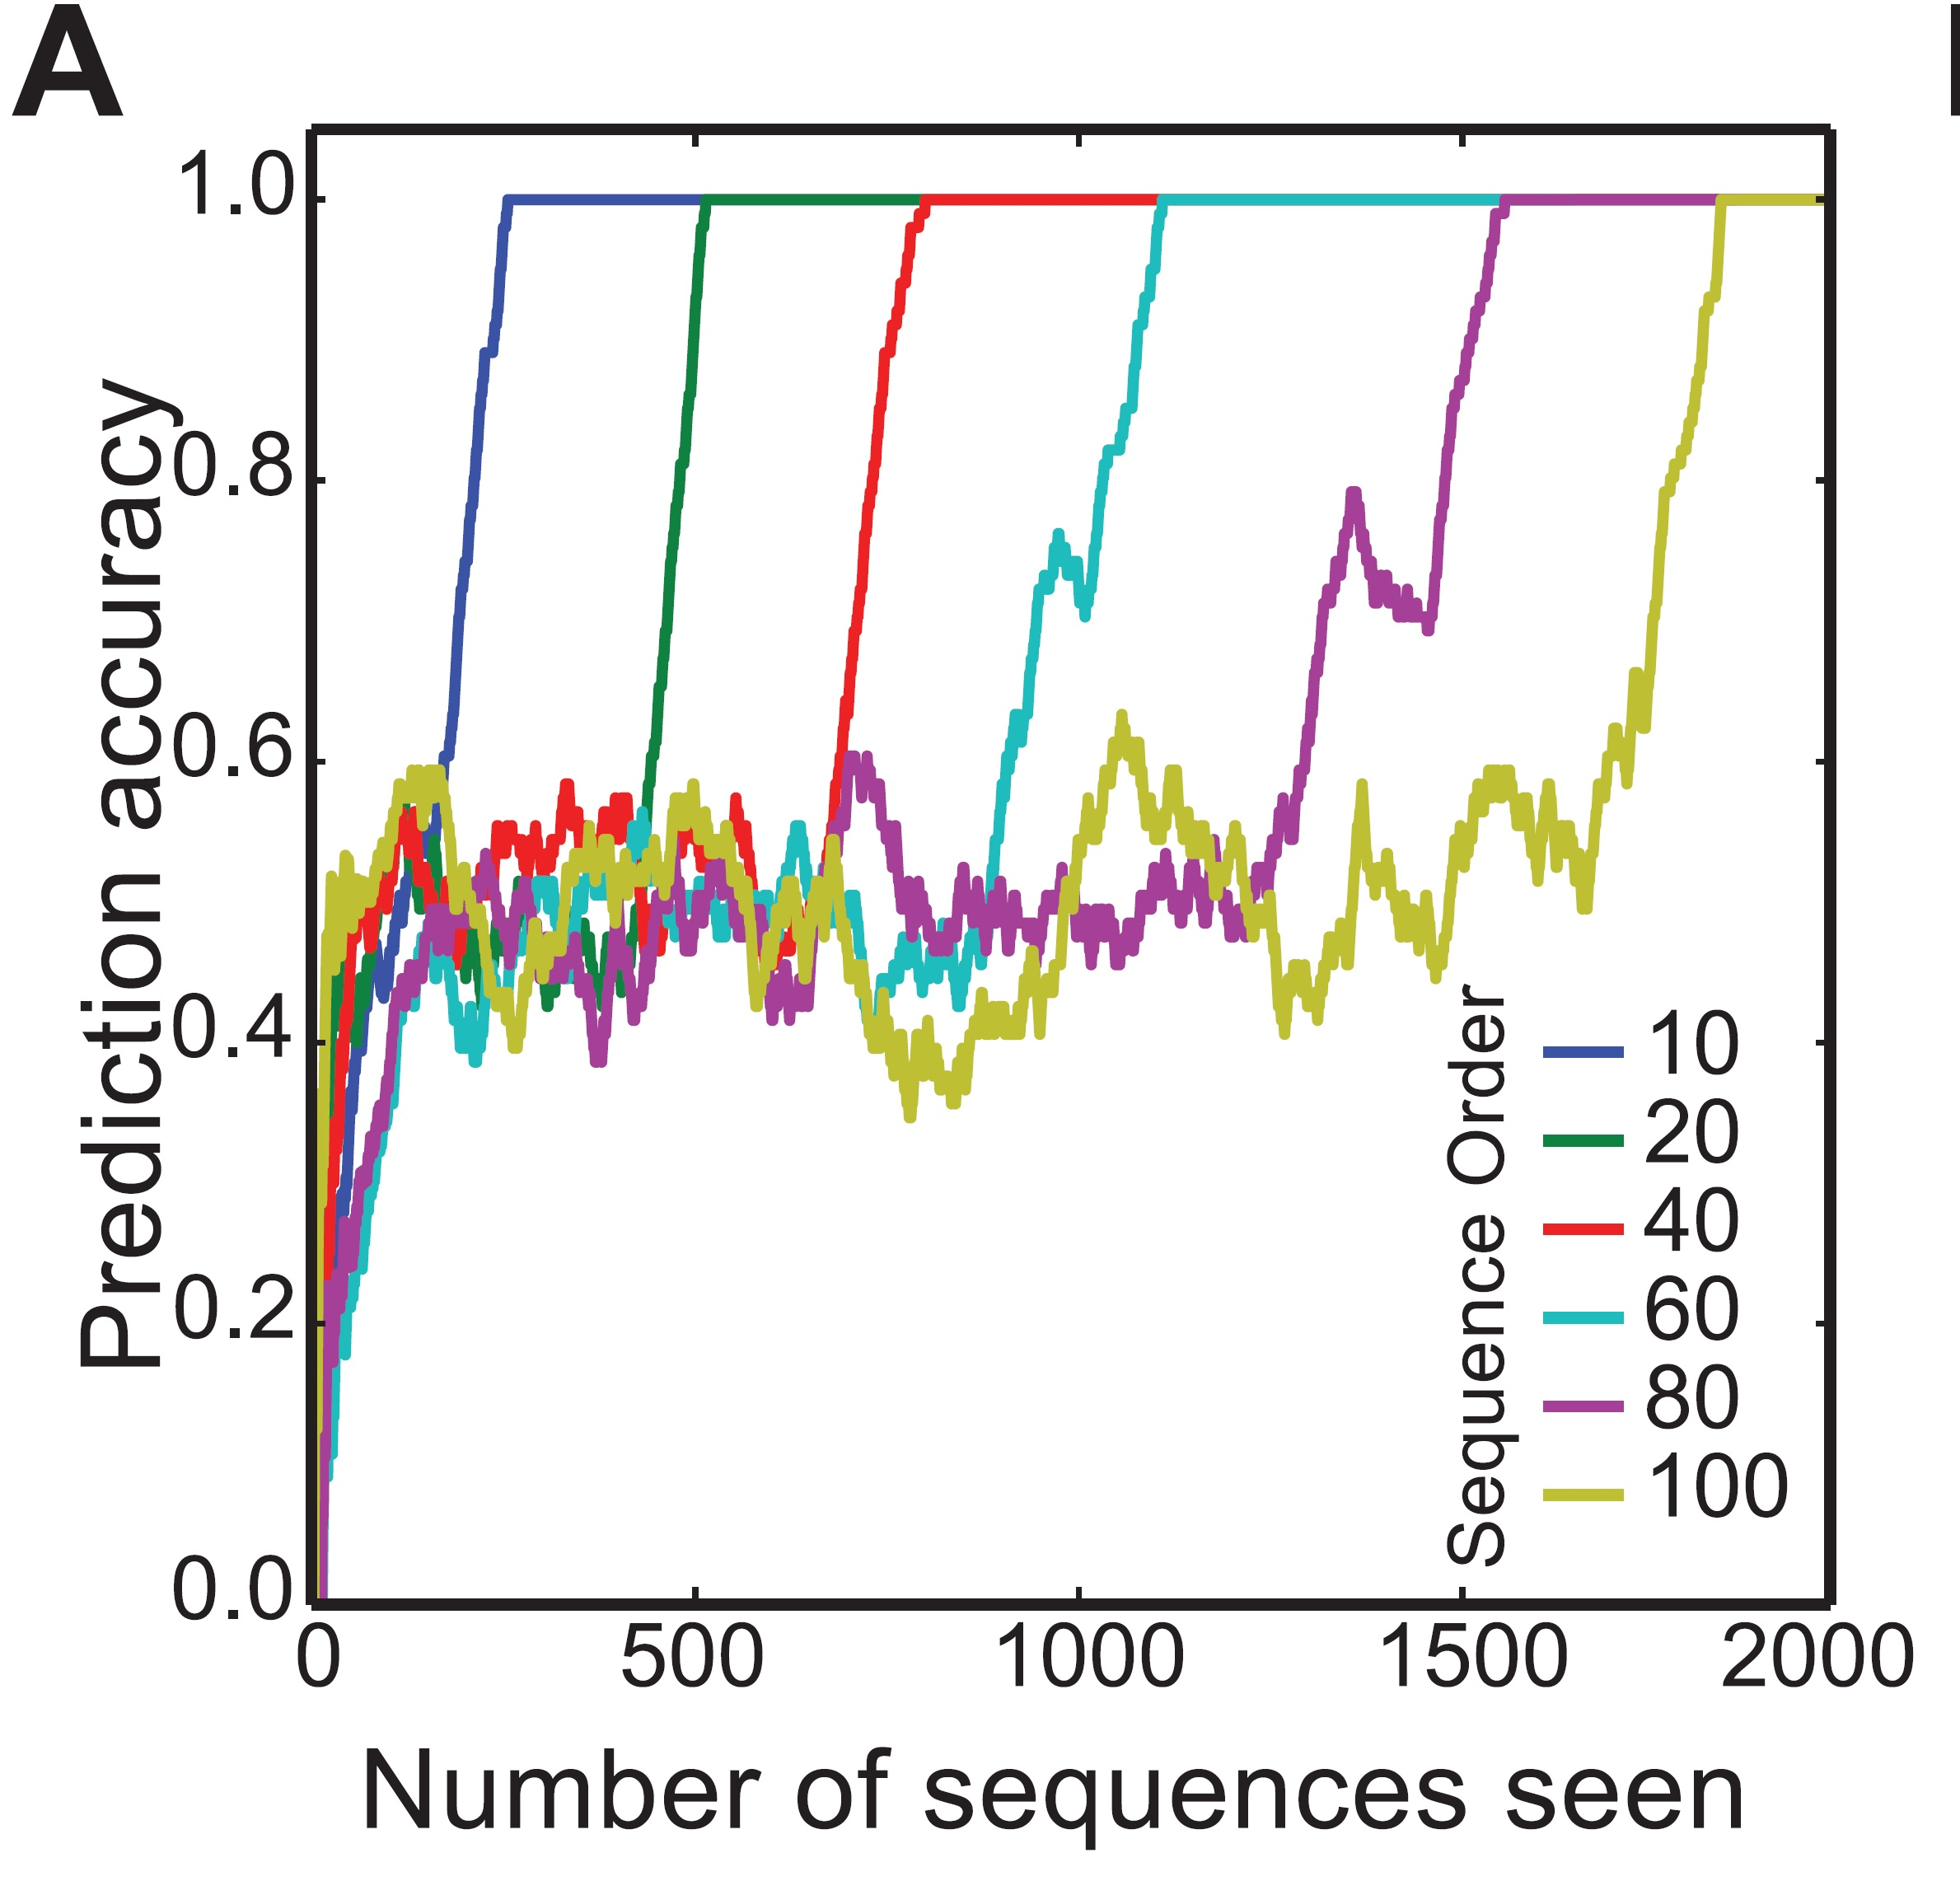
\includegraphics[width=0.6 \textwidth,center]{../pics/sequence_order.jpg}}
	\vspace{0.5em}
	\visible<2->{
	  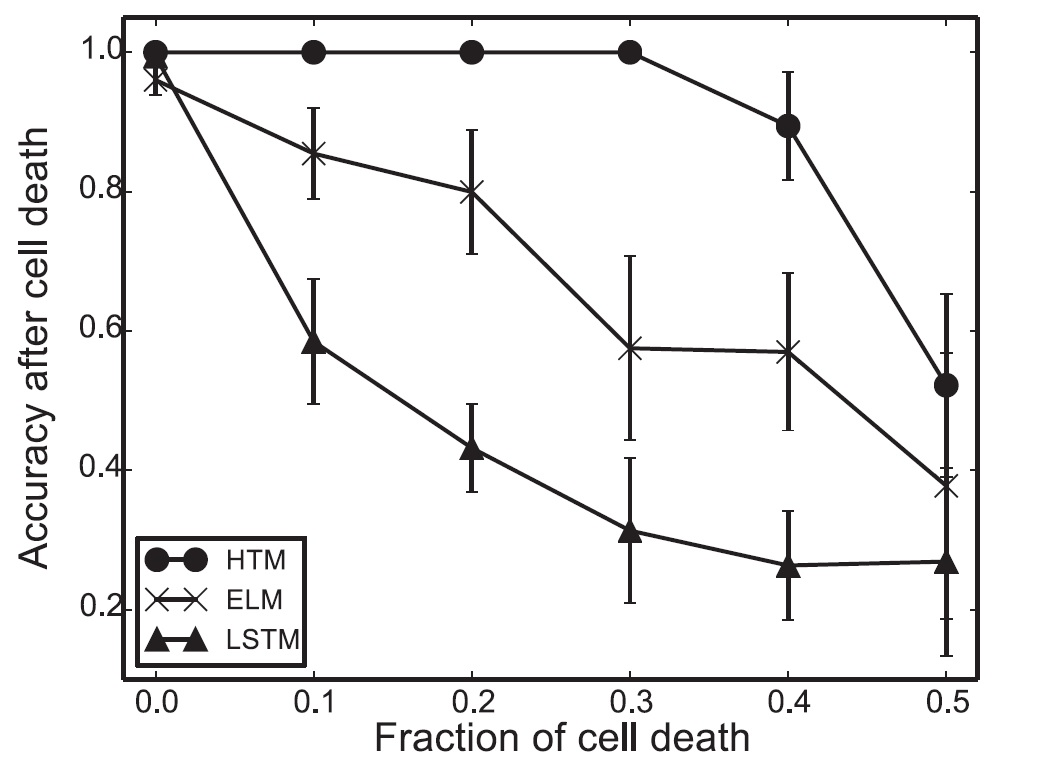
\includegraphics[width=0.65 \textwidth,center]{../pics/cell_death.jpg}}
  \end{columns}
\end{frame}

\begin{frame}{Πραγματικά δεδομένα}
  Ζήτηση ταξί Νέας Υόρκης (διάστημα 30 λεπτών) \tiny{\cite{continuous}}
  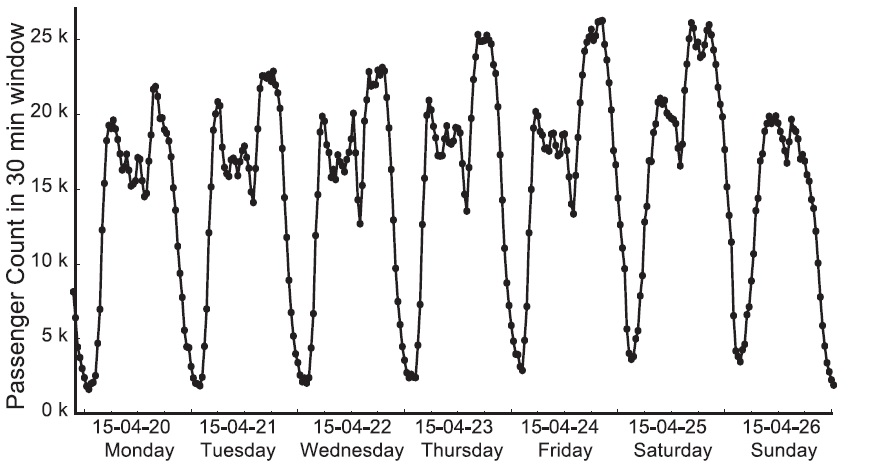
\includegraphics[width=0.5 \textwidth,center]{../pics/taxi_demand.jpg}
  \vfill
  \pause
  \begin{columns}
	\column {0.5 \textwidth}
	Στόχος: Πρόβλεψη της ζήτησης 2.5 ώρες πριν
	\column {0.4 \textwidth}
	\vspace{1em}
	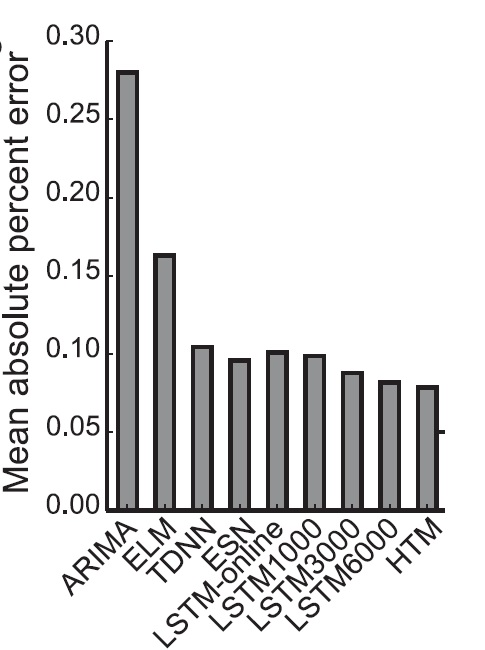
\includegraphics[width=0.6 \textwidth,left]{../pics/taxi_accuracy.jpg}
  \end{columns}
\end{frame}


\section{Hardware}

\begin{frame}{SpiNNaker Chip}
  Yψηλής παραλληλοποίησης υπολογιστικό σύστημα για την μοντελοποίηση και προσομοίωση spiking 				neural networks.
  \pause
  \vfill
  Βασικό στοιχείο το SpiNNaker Chip Multiprocessor (CMP) \tiny{\cite{spinnaker}}:
  \vfill
  \begin{columns}
	\column{0.5 \textwidth}
	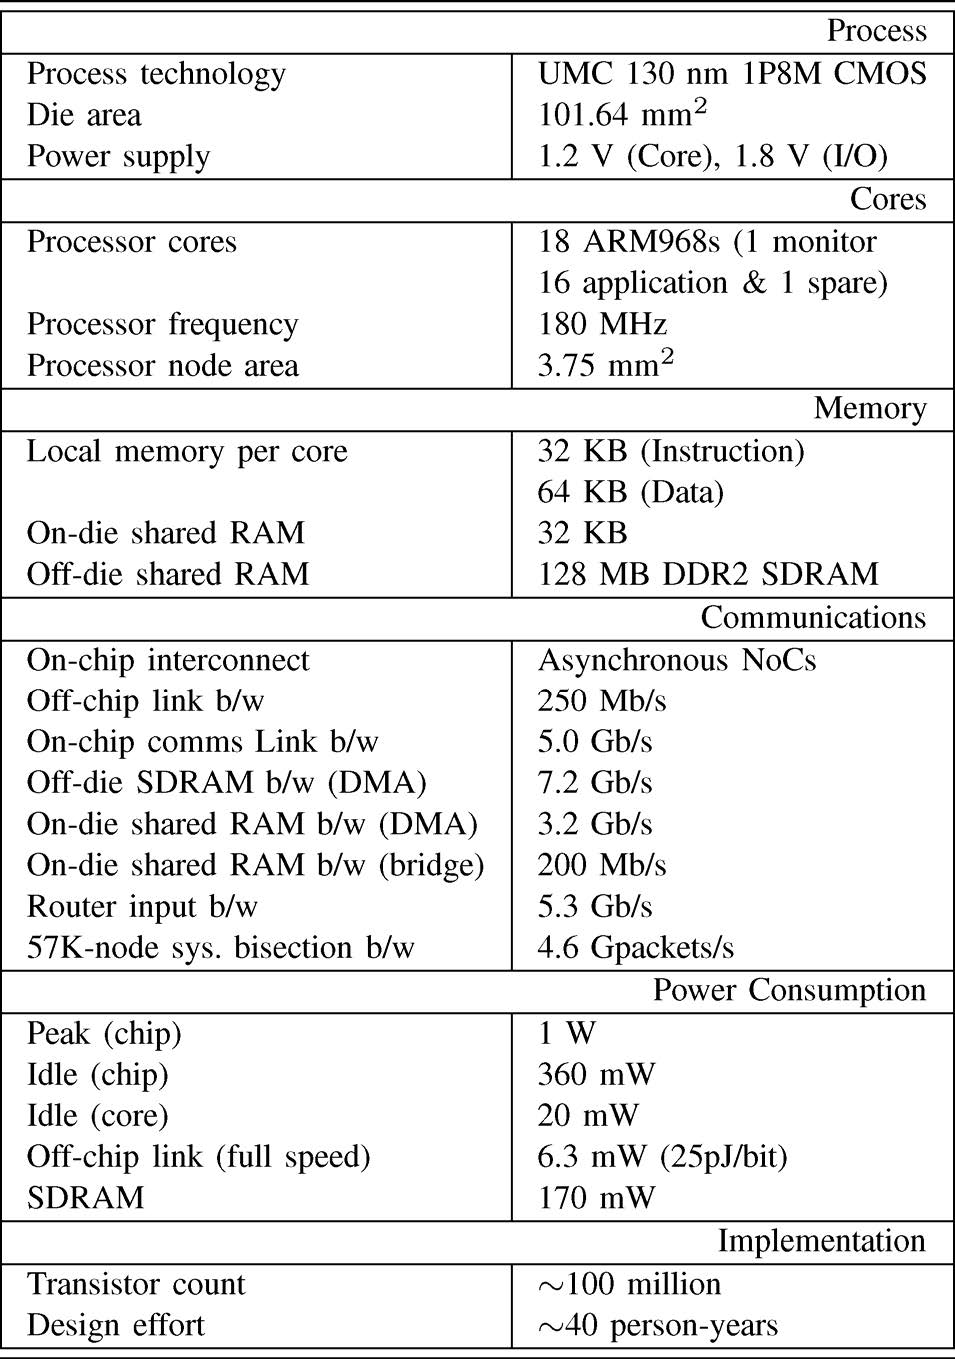
\includegraphics[width=0.75 \textwidth,right]{../pics/CMPspecs.jpg}
	\column{0.5 \textwidth}
	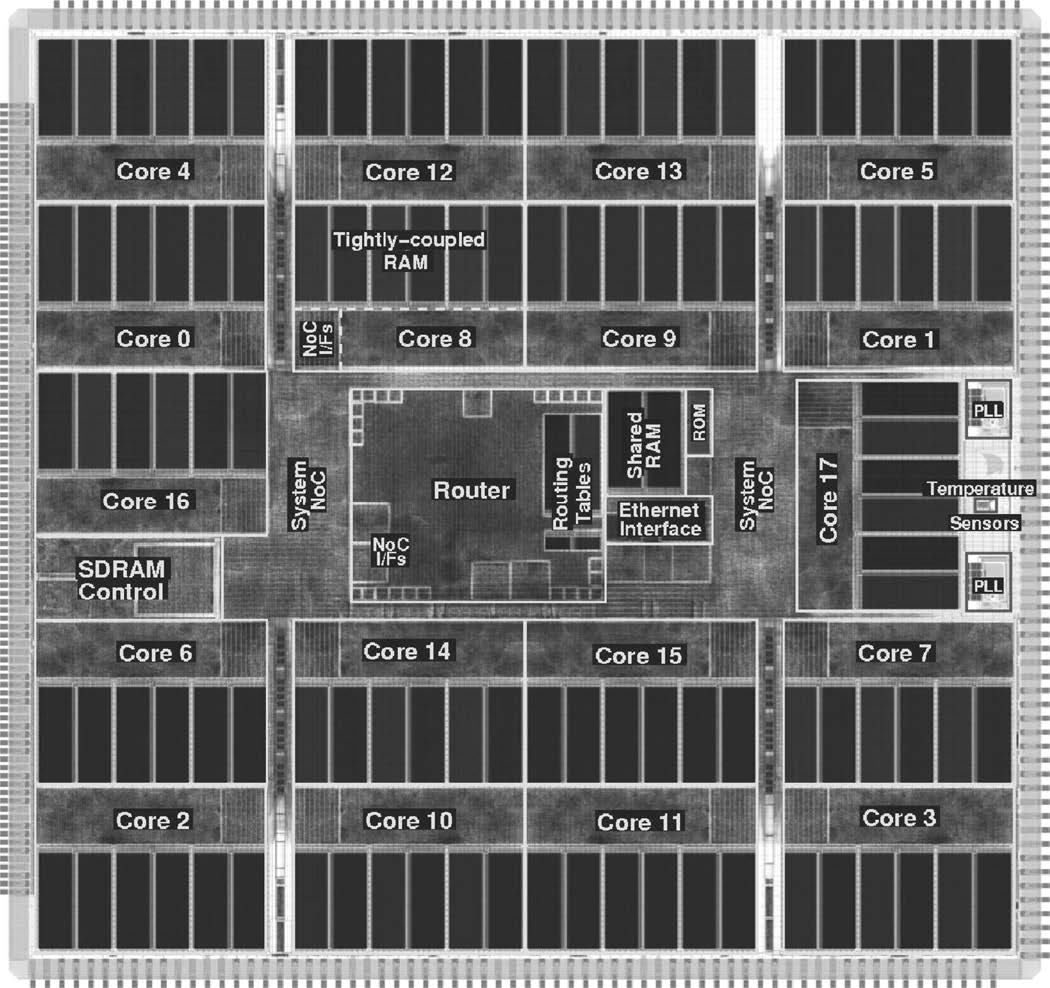
\includegraphics[width=0.75 \textwidth,left]{../pics/CMP.jpg}
  \end{columns}
\end{frame}

\begin{frame}{SpiNNaker Network}
  SpiNNaker: Πίνακας από κόμβους που περιέχουν CMP και 128MB SDRAM σε κοινό package.
  \pause
  \vfill
  Συνολικά, έχουμε:
  \begin{columns}
	\column{0.6 \textwidth}
	  \begin{itemize}
		\item[--] 57600 CMPs
		\item[--] $10^6$ ARM968
		\item[--] $10^{9}$ νευρώνες ($1 \%$ εγκεφάλου)
		\item[--] 228 TIPS
		\item[--] 90KW ισχύς
	  \end{itemize}
	\column{0.5 \textwidth}
	  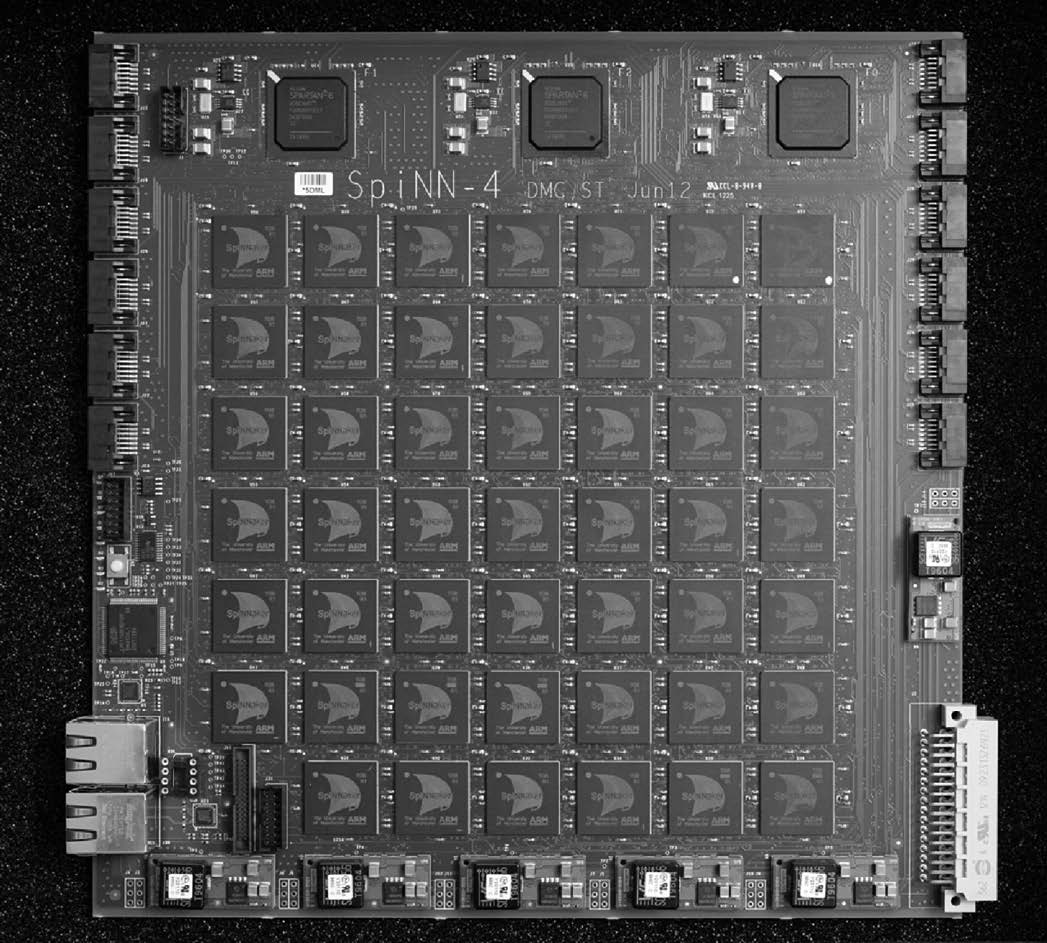
\includegraphics[width=0.9 \textwidth,left]{../pics/Spinnaker.jpg}
  \end{columns}
\end{frame}

\begin{frame}{Χαρακτηριστικά SpiNNaker}
  \begin{description}[Sensor output]
	\item[Επικοινωνία] Address Event Representation (AER), NoC
	  \pause
	  \vfill
	\item[Μνήμη] Fast-access για την κατάσταση του νευρώνα\\
	  SDRAM για την κατάσταση των συνάψεων
	  \pause
	  \vfill
	\item[Κατανάλωση] Ασύγχρονη Επικοινωνία\\
	  Sleep mode στην idle κατάσταση \\
	  Επιλογή ARM968 και SDRAM
  \end{description}
\end{frame}

\begin{frame}{Παράδειγμα υλοποίησης}
  Σύστημα για classification χειρόγραφων ψηφίων (MNIST database) μέσω Deep Neural Network
  \vspace{1em}
  \pause
  \begin{columns}
	\column {0.4 \textwidth}
	\begin{itemize}
	  \item<2->[--] Ακρίβεια
	  \item<3->[--] Ισχύς: 0.3 Watt
	  \item<4->[--] Latency
	\end{itemize}

	\column {0.6 \textwidth}
	\visible<2->{
	  \\
	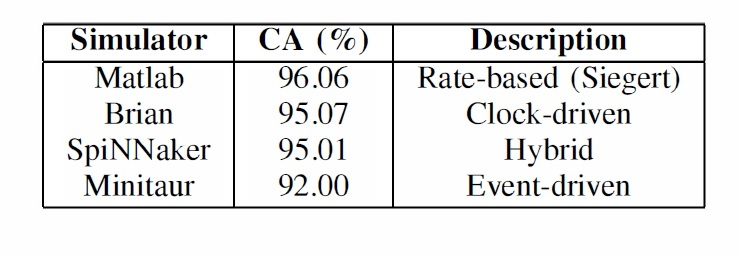
\includegraphics[width=0.8 \textwidth,left]{../pics/Accuracy.jpg}
	}
	\vspace{0em}
	\visible<4->{
	  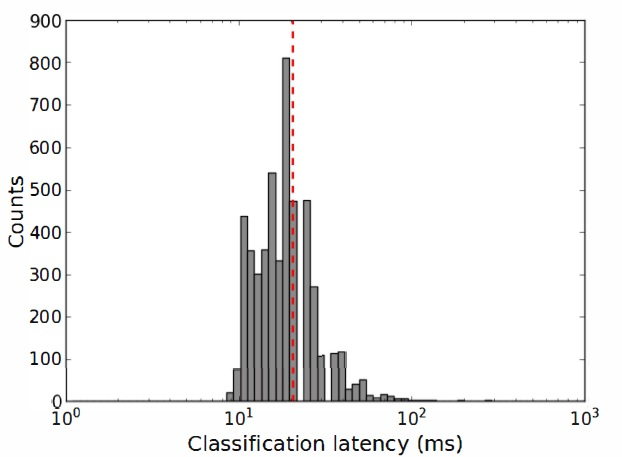
\includegraphics[width=0.8 \textwidth,left]{../pics/Latencies.jpg}
	}
  \end{columns}
\end{frame}

\begin{frame}{BrainScaleS Project (BSS)}
  Υβριδική πλατφόρμα: Cluster + Νευρομορφικό σύστημα
  \vfill
  \pause
  Βασικό στοιχείο: High Input Count Analog Neural Network (HICANN) \tiny{\cite{wafer}}
  \vfill
  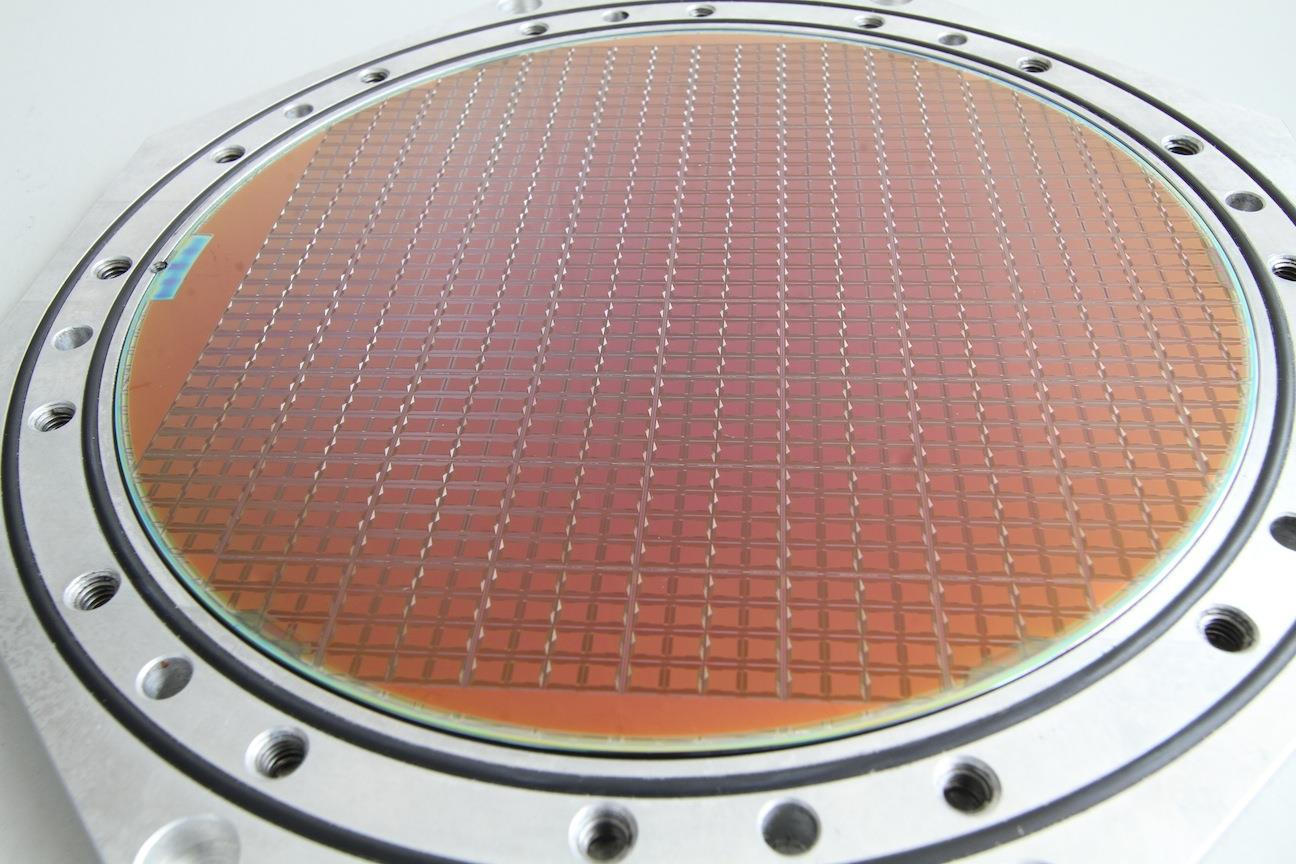
\includegraphics[width=0.4 \textwidth,center]{../pics/HICANN.jpg}
  \pause
  \vfill
  Mixed-signal: Αναλογικά νευρωνικά κυκλώματα, Ψηφιακή επικοινωνία
\end{frame}

\begin{frame} {HICANN Chip}
  Κάθε HICANN chip \tiny{\cite{wafer}}:
  \begin{itemize}
	\item[--] 512 νευρώνες τύπου AdEx
	\item[--] 2 ομάδες 226 συνάψεων (πχ. proximal, distal)
  \end{itemize}
  \pause
  \vfill
  Ένα wafer περιέχει $364$ HICANN chips, δηλαδή:
  \begin{itemize}
	\item[--] $200\cdot 10^3$ νευρώνες
	\item[--]$45\cdot 10^6$ συνάψεις
  \end{itemize}
  \pause
  \vfill
  Η σημερινή πλατφόρμα αποτελείται 20 wafers.

\end{frame}

\begin{frame} {HICANN Chip}
  \begin{columns}
	\column {0.5 \textwidth}
	\begin{itemize}
	  \item<1->[--]Motherboard πάνω\\ από το wafer
	  \item<1->[--]FPGA για inter-wafer επικοινωνία
	\end{itemize}
	\vspace{5em}
	\begin{itemize}
	  \item<2->[--]Διαχωρισμός σε reticles
	  \item<2->[--]Συνδέσεις μέσω πυκνού δικτυώματος από wires
	\end{itemize}

	\column {0.5 \textwidth}
	\visible<1->{
	  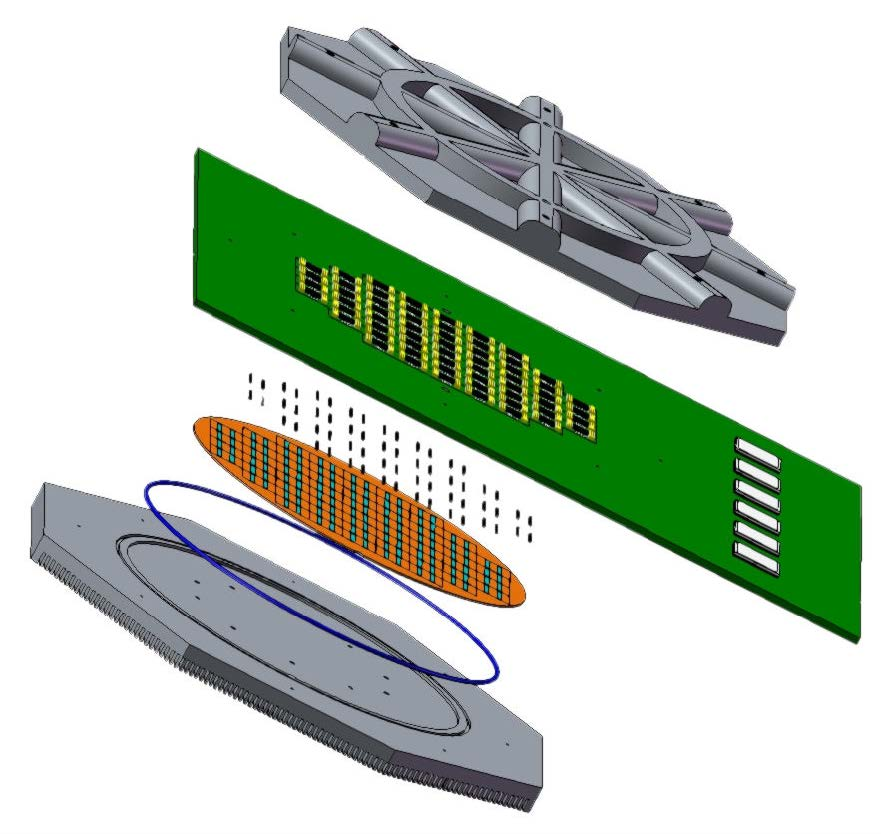
\includegraphics[width=0.7 \textwidth,left]{../pics/wafer.jpg}}
	\vspace{1em}
	\visible<2->{
	  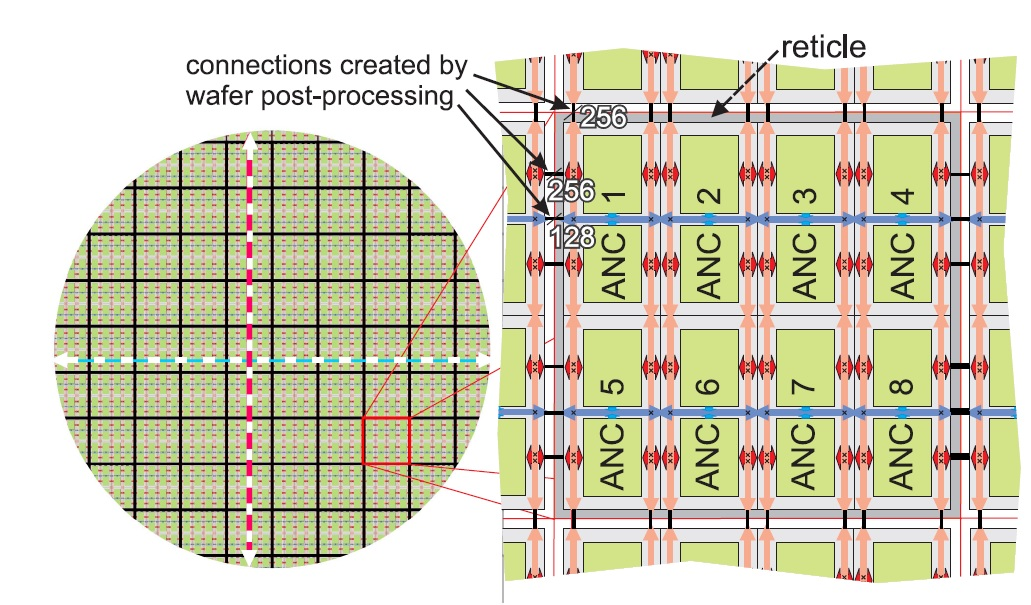
\includegraphics[width=0.8 \textwidth,left]{../pics/reticle.jpg}}
  \end{columns}
\end{frame}

\begin{frame} {HICANN Chip}
  \begin{columns}
	\column {0.5 \textwidth}
	\begin{itemize}
	  \item<1->[--] Κυκλώματα μεμβράνης
	  \item<2->[--] Είσοδος από synapse driver
	  \item<3->[--] Strobe lines
	  \item<4->[--] Neuron builder
	\end{itemize}
	\column {0.6 \textwidth}
	\visible<1->{
	  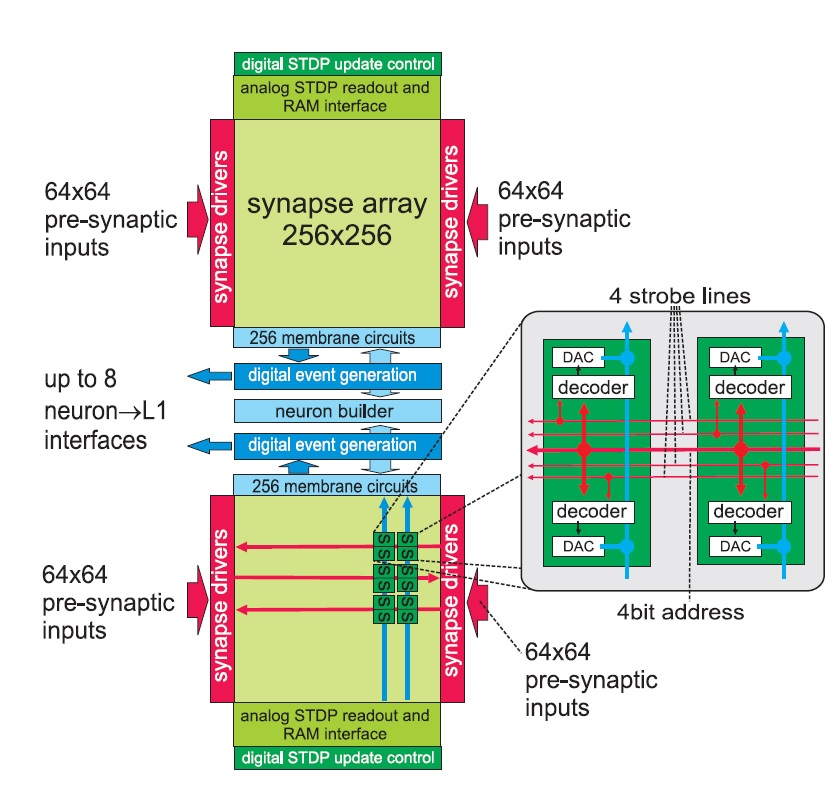
\includegraphics[width=0.9 \textwidth,left]{../pics/insideHICANN.jpg}}
  \end{columns}
\end{frame}

\begin{frame}{Συνάψεις}
  \begin{itemize}
	\item<1->[--]4 bit SRAM για το βάρος
	\item<1->[--]Ρεύμα ανάλογο του βάρους
	\item<1->[--]MUX για επιλογή εισόδου (excitatory/inhibitory)
  \end{itemize}
  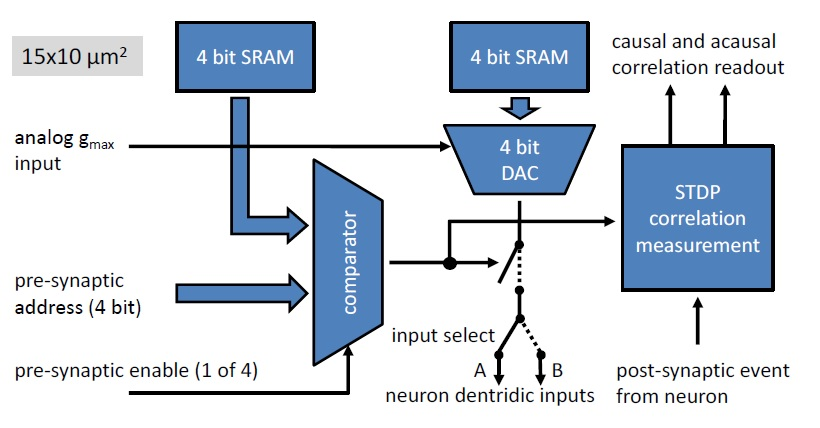
\includegraphics[width=0.8 \textwidth,center]{../pics/synapses.jpg}
\end{frame}

\begin{frame}{Adaptive Exponential Model}
  \begin{tabbing}
	To AdEx περιγράφεται από 2 μεταβλητές:  \=α) Δυναμικό Μεμβράνης\\
	  \>β) Adaptation w
  \end{tabbing}
	  \pause
	  Σε DC είσοδο παρουσιάζει την εξής συμπεριφορά:
	  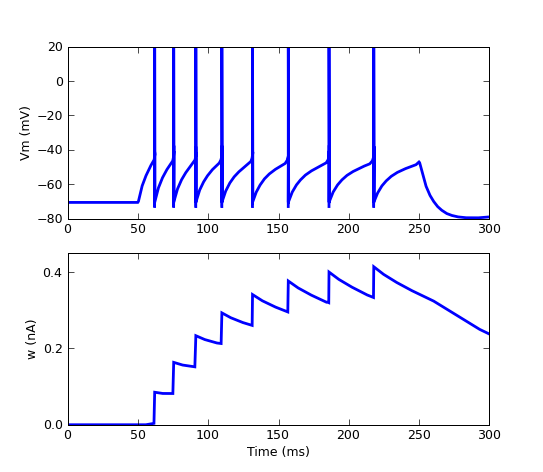
\includegraphics[width=0.4 \textwidth,center]{../pics/adex.jpg}
	  \pause
	  \vfill
	  Tο rise time εξαρτάται από το επίπεδο του input.

\end{frame}

\begin{frame}{Υλοποίηση Spatial Pooler \tiny{\cite{htmheidelberg}}}
  Time - based σύστημα: Οι νευρώνες με το μεγαλύτερο input ενεργοποιούνται πρώτοι\\
  \vspace{2em}
  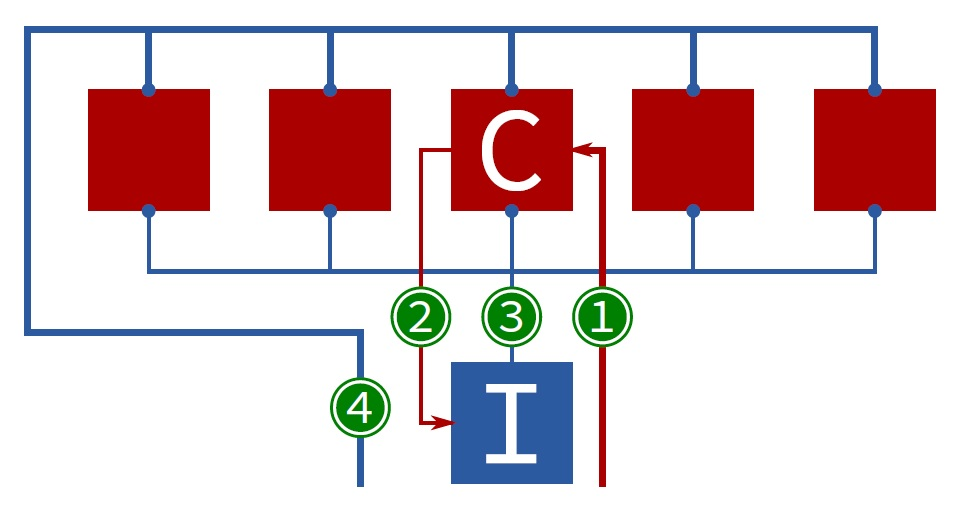
\includegraphics[width=0.5 \textwidth,center]{../pics/spatial_hardware.jpg}
  \pause
  \vfill
  \begin{tabbing}
	Το inhibition cell(I):  \= α) διατηρεί τo sparsity\\
	  \> β) ελέγχει τη σταθερότητα\\
  \end{tabbing}
\end{frame}

\begin{frame}{Υλοποίηση Temporal Pooler \tiny{\cite{htmheidelberg}}}
  \begin{columns}
	\column {0.6\textwidth}
	\begin{itemize}
	  \item<1->[--] Ένα κελί (P) για το proximal input
	  \item<1->[--] Μια τριάδα (D,I,S) για κάθε νευρώνα του multicolumn
		\vspace{1em}
	  \item<2->[--] To Distal (D) αθροίζει τις συνάψεις "πρόβλεψης"
		\vspace{1em}
	  \item<3->[--] Το Inhibition (I) καθορίζει ποιοι νευρώνες του ενεργού multicolumn 							ενεργοποιούνται
	\end{itemize}

	\column {0.4\textwidth}
	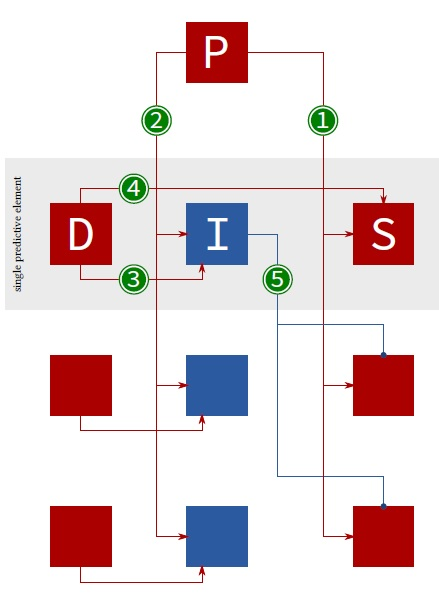
\includegraphics[width=1 \textwidth,center]{../pics/temporal_hardware.jpg}
  \end{columns}

\end{frame}

\begin{frame}{Αποτελέσματα προσομοιώσεων}
  \begin{columns}
	\column {0.5 \textwidth}
	\begin{itemize}
	  \item<1->[--]Ενεργοποίηση νευρώνων με μεγαλύτερο overlap
	\end{itemize}
	\vspace{5em}
	\begin{itemize}
	  \item<2->[--]Διατήρηση συσχετίσεων εισόδου-εξόδου
	\end{itemize}

	\column {0.5 \textwidth}

	\visible<1->{
	  \vspace{1em}
	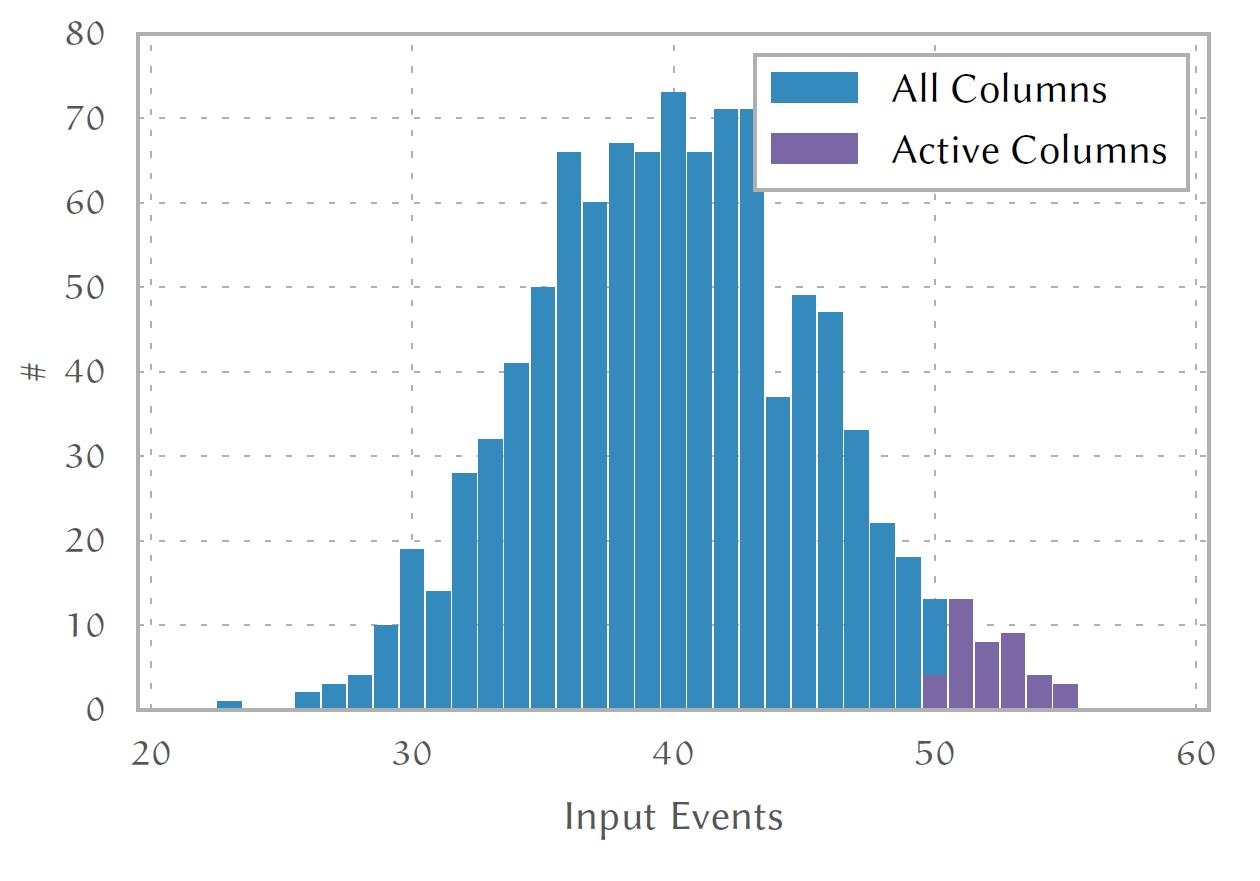
\includegraphics[width=0.9 \textwidth,left]{../pics/spatialsim1.jpg}}
  \vspace{0.5em}
	\visible<2->{
	  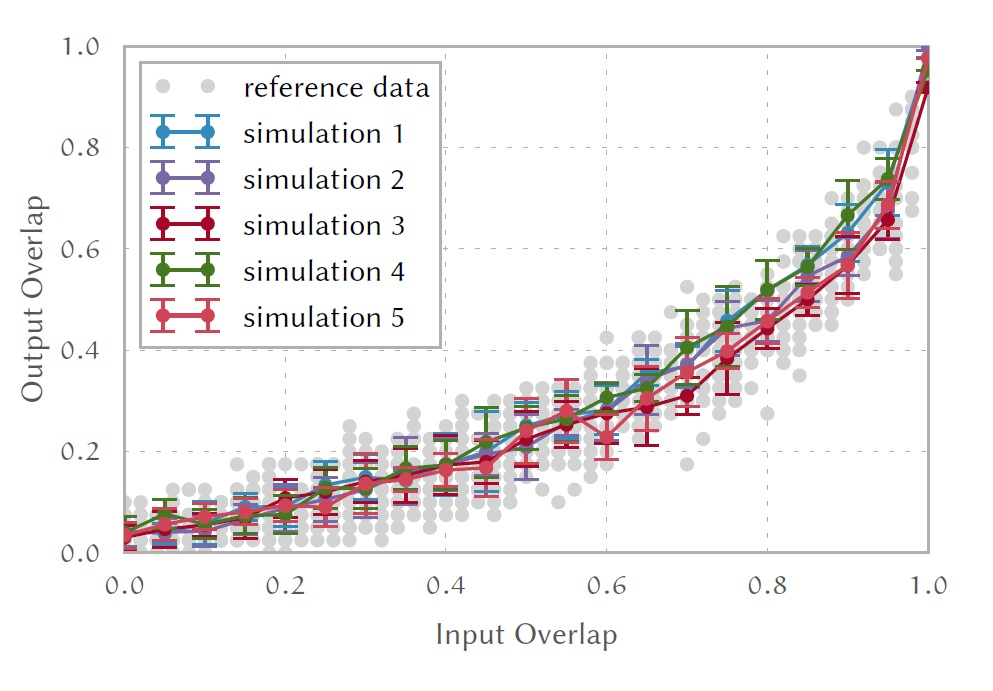
\includegraphics[width=0.9 \textwidth,left]{../pics/spatialsim2.jpg}}
  \end{columns}
\end{frame}

\nocite{*}
\begin{frame}[plain,allowframebreaks]
  \printbibliography
\end{frame}

\begin{frame}
  \centering
  \vspace{3em}
  
\includegraphics[width=.55\textwidth]{../pics/thanks}
\end{frame}

\end{document}
